%%%% Tesis%%%%
\documentclass[12pt,a4paper]{book}

% \usepackage[T1]{fontenc}
\usepackage[utf8]{inputenc}
\usepackage{amsmath}       % innecesarios si se usa amsart/amsbook % USO
% \usepackage{amsfonts}
\usepackage{amssymb} % USO
\usepackage{bold-extra}
% \usepackage{amsthm}
\usepackage{latexsym}
\usepackage{emptypage}
% \usepackage{graphicx} % USO
% \usepackage{wrapfig}
% \usepackage{rotating}
\usepackage[section]{placeins}
\usepackage[usenames, dvipsnames]{color} % USO
% \usepackage{colortbl}
% \usepackage{flafter}
% % \usepackage{subfigure} % USOD
\usepackage{fancyhdr}
\usepackage{pdfpages}
% \usepackage{natbib}
% \usepackage[margin=20pt, font=small, labelfont=bf, labelsep=period]{caption}
% \usepackage{url}             % espaciado adecuado de las URL largas en las referencias
%\usepackage{path}            % espaciado y guinado adecuado para las rutas de directorios
% \usepackage[final]{listings} % codigo fuente
% \usepackage{appendix}        % mejor control sobre los apendices
% \usepackage{amsmath,amsthm,amstext,amssymb,amsfonts}
\usepackage{textcomp}   % extra symbols (textopenbullet) % USO

% \usepackage{rotating}

% \usepackage{tabularx}
% \usepackage{booktabs}
% 
\usepackage{etoolbox, tocloft}
%\patchcmd{\tableofcontents}{\MakeUppercase\contentsname}{\contentsname}{}{}
\preto\section{%
  \ifnum\value{section}=0\addtocontents{toc}{\vskip10pt}\fi
}
\preto\figure{%
  \ifnum\value{figure}=0\addtocontents{lof}{{\bfseries Chapter \thechapter\vskip10pt}\par}\fi
}
\preto\table{%
  \ifnum\value{table}=0\addtocontents{lot}{{\bfseries Chapter \thechapter\vskip10pt}\par}\fi
}

\usepackage[pagebackref=true]{hyperref}
\hypersetup{colorlinks=true, linkcolor=black, citecolor=black, filecolor=black, urlcolor=black, linktoc=page,
	pdftitle={End-to-end modelling approach for an ecosystem approach to fisheries in the Humboldt Current Ecosystem}, 
	pdfauthor={Ricardo Oliveros--Ramos}, 
	pdfsubject={PhD Thesis},
pdfkeywords={Ecosystem modelling, Humboldt Current Ecosystem, OSMOSE}}

\usepackage{cite} % CREO QUE USO
\usepackage[round]{natbib} % USO
\usepackage{lscape} % USO
\usepackage{multirow} % USO
\usepackage{csquotes}
% \usepackage{subfig} % USO
\usepackage{caption}
\usepackage{subcaption}
% \renewcommand\thesubfigure{\roman{subfigure}}
\usepackage{array,graphicx}
\usepackage{booktabs}
\usepackage{threeparttable}
% \usepackage{biblatex}
% \usepackage[backend=biber,style=authoryear,sortcites,sorting=ynt]{biblatex}
% \addbibresource{referencesthese.bib}
\usepackage{appendix}
\usepackage{setspace}
\usepackage{titlesec}
\usepackage{lipsum}

\newcommand*\rot{\rotatebox{90}}


% \bibliographystyle{authordate_perso.bst}
%\bibliographystyle{ecology_rocio.bst}
% \bibliographystyle{te.bst}
%\graphicspath{{/data/rociocokriging/}{/data/mes_images/}}

%% Maquetacion ------------------------------------------------------------
   \parskip 0cm
   \oddsidemargin 2cm
   \evensidemargin 2cm
   \topmargin 1cm
   \textheight 23.5cm
   \textwidth 15cm
   \voffset -1.5cm
   \hoffset -2cm
   \headheight 1cm
   \headsep 1cm
   \topskip 0cm
   
% 
% \setlength{\oddsidemargin}{35mm}
% \setlength{\evensidemargin}{25mm}
% \setlength{\voffset}{-0.725in}
% \setlength{\hoffset}{-1in}
% \setlength{\textwidth}{150mm}
% \setlength{\topmargin}{4mm}
% \setlength{\headheight}{10mm}
% \setlength{\headsep}{15mm}
% \setlength{\topskip}{0mm}
% \setlength{\textheight}{243mm}

% \renewcommand{\baselinestretch}{1.2}           % interlinado un poquito m�s amplio
\setstretch{1.25}


% incluir numero de capitulo en las numeraciones
\numberwithin{section}{chapter}
\numberwithin{equation}{chapter}
\numberwithin{figure}{chapter}
\numberwithin{table}{chapter}



% definitions
\newcommand{\RR}{\mathbb{R}}
\def\xpar{\tilde{x}}
\def\xmean{x_k}
\def\smean{\sigma_k}
\def\xdyn{\textbf{x}_k}
\def\sdyn{\textbf{s}_k}
\def\smax{\textbf{s}^{(\max)}_k}
\def\smin{\textbf{s}^{(\min)}_k}
\def\xfinal{\textbf{x}}
\def\sfinal{\textbf{s}}
\def\ccov{c_{cov}}
\def\mucov{\mu_{cov}}
\def\step{\sigma_{size}}

% % comandos
% \newcommand{\ve}[1]{\boldsymbol{#1}}                       % vectores
% \newcommand{\mat}[1]{\boldsymbol{\mathsf{#1}}}          % matrices (roman)
% \newcommand{\esp}[1] {\mathbb{E}\left[#1\right]}	% esperanza
% \newcommand{\var}[1] {\mathbb{V}\left[#1\right]}	% varianza
% \newcommand{\cov}[1] {\mathbb{C}\left[#1\right]}	% funci�n de covarianza
% \newcommand{\pr}[1] {\mathbb{P}\left[#1\right]}		% Probabilidad
% \newcommand{\alert}[1]{\noindent\textcolor{BrickRed}{\textbf{(#1)\\}}}
% \newcommand{\simiid}{\buildrel\rm iid \over\sim}        % ~ iid
% \newcommand{\R}{\texttt{R}}
% \newcommand{\inla}{\texttt{INLA}}
% 
% \DeclareMathOperator{\logit}{logit}
\DeclareMathOperator*{\argmax}{arg\,max}
% 
% \newcommand{\af}{\alpha}
% \newcommand{\ta}{\theta}
% \newcommand{\ld}{\lambda}
% \newcommand{\M}{I\!\!M}
% \newcommand{\I}{\mathbb I}
% \newcommand{\1}{\mathbf{1}}
% \newcommand{\pp}{\Phi}
% \newcommand{\N}{\mathbb N}
% \newcommand{\x}{{\bf x}}
% \newcommand{\argmax}{\mbox{ argmax}}
% \renewcommand{\topfraction}{0.85}
% \renewcommand{\textfraction}{0.1}
% \newcommand{\dd}{\mathrm{d}}
% \newcommand{\T}{{\sf{T}}}
% \newcommand{\vecx}{\mathbf{x}}
% \newcommand{\vecy}{\mathbf{y}}
% \newtheorem{definition}{Definition}
% \newenvironment{example}{\noindent{\bf Example\/} \rm}{\hfill \\}
% \newenvironment{remark}{\noindent{\bf Remark\/} \rm}{\hfill \\}
% 
% \def\mm#1{\ensuremath{\boldsymbol{#1}}} % version: amsmath

%% Comandos necesarios para hacer el glosario
%\def\glossaryname{Glosario de s\'{\i}mbolos}
%\makeglossary
% 
% % This is done with the titlesec package                                                                            
%   \titleformat{\chapter}[hang]
% 	      {\thispagestyle{empty}}
%               {\normalfont\Large\filcenter} % {fmt}                                                                   
%               {\thechapter.\ }              % {label}                                                                 
%               {1pc}                         % {sep}                                                                   
% %               {\vspace{-1in}\enlargethispage{-0.5in}\thispagestyle{empty}}    % {before}                                  
% % 



\pagestyle{fancy}

 \fancyhead{}
        \fancyfoot{}
        \fancyhead[LO]{\rightmark}
        \fancyhead[RE]{\leftmark}
        \fancyhead[LE,RO]{\thepage}
        \renewcommand{\chaptermark}[1]{\markboth{\thechapter.\ #1}{}}
        \renewcommand{\sectionmark}[1]{\markright{\thesection\ #1}}

%
%\makeatletter
%\if@twoside
%  \renewcommand*{\chaptermark}[1]{%
%    \markboth{%
%      \ifnum\value{secnumdepth}>-1 %
%        \thechapter\ %
%      \fi
%      #1%
%    }{}%
%  }%
%\else
%  \renewcommand*{\chaptermark}[1]{%
%    \markright{%
%      \ifnum\value{secnumdepth}>-1 %
%        \if@mainmatter  
%          \thechapter\ %
%        \fi
%      \fi
%      #1%
%    }%
%  \fi
%\makeatother

% my new commandas

\newcommand{\includepaper}[1]{
\cleardoublepage
\setlength{\voffset}{0cm}
\setlength{\hoffset}{0cm}
\newpage
\includepdf[pages=-]{#1}
\setlength{\voffset}{-1.5cm}
\setlength{\hoffset}{-2cm}
\clearpage	
}

\newcommand{\includeappendix}[1]{
\clearpage
\setlength{\voffset}{0cm}
\setlength{\hoffset}{0cm}
\newpage
\includepdf[pages=-]{#1}
\setlength{\voffset}{-1.5cm}
\setlength{\hoffset}{-2cm}
\clearpage	
}

\begin{document}

\frontmatter

\begin{titlepage}
\setstretch{1.1}
\begin{center}
  
\vspace*{-0.08\textheight}


\includegraphics[width=0.2\textwidth]{figures/um2.png}\hfill
\includegraphics[width=0.19\textwidth]{figures/imarpe.png}\hfill

\includegraphics[width=0.2\textwidth]{figures/ird.png}

\vspace*{.03\textheight}
\begin{center}
{\LARGE \textbf{TH\`{E}SE DE DOCTORAT}}\\
\end{center}

\vspace*{.005\textheight}
\begin{center}
{\large \'{E}cole Doctorale SIBAGHE - Syst\`{e}mes int\'{e}gr\'{e}s en Biologie, Agronomie, G\'{e}osciences, 
Hydrosciences et Environnement}\\[.01\textheight]
{Sp\'{e}cialit\'{e} : Evolution, Ecologie, Ressources G\'{e}n\'{e}tiques, Pal\'{e}ontologie}

\end{center}

\vspace*{.005\textheight}
\begin{center}
{\large Pr\'{e}sent\'{e} par :\\ David Ricardo \textsc{Oliveros Ramos}}
\end{center}

\vspace*{.005\textheight}
\begin{center}
{\large Pour obtenir le grade de :\\ \textsc{Docteur de l'Universit\'{e} de Montpellier 2}}
\end{center}

\vspace*{.005\textheight}
\begin{center}
{\large Sujet de la th\`{e}se :}
\end{center}

% \vspace*{.005\textheight}
\begin{center}
\large{\bf End--to--end modelling for an ecosystem approach to fisheries in the Northern Humboldt Current Ecosystem}\\
\end{center}
% \

% \vspace*{.01\textheight}
\begin{center}
\large{Mod\'{e}lisation ``end--to--end'' pour une approche \'{e}cosyst\'{e}mique des p\^{e}ches dans le Nord courant de Humboldt}\\
\end{center}

\vspace*{.015\textheight}
\begin{center}
{\large Soutenue le \textbf{8 decembre 2014} devant le jury compos\'{e} de : }
\end{center}


\begin{tabular}{lr}
\textbf{Yunne-Jai \textsc{Shin}}, IRD, France. & Directrice de th\`{e}se\\
\textbf{Arnaud \textsc{Bertrand}}, IRD, France. & Co-directeur de th\`{e}se\\
\textbf{Stephanie \textsc{Mahevas}}, IFREMER, France. & Rapportrice\\
\textbf{Jean-Christophe \textsc{Poggiale}}, AMU, France. & Rapporteur\\
\textbf{Ray \textsc{Hilborn}}, University of Washington, USA. & Examinateur\\
\textbf{Philippe \textsc{Cury}}, IRD, France. & Examinateur\\
\textbf{Jorge \textsc{Csirke}}, FAO, Per\'u. & Examinateur (invit\`{e})\\
\textbf{Coleen \textsc{Moloney}}, UCT, South Africa. & Examinateur (invit\`{e})\\
\end{tabular}

%\vfill

%% Bottom of the page
%{\large \today}

\end{center}

\end{titlepage} \thispagestyle{empty}

%%%%%%%%%%%%%%%%%
\cleardoublepage

\setcounter{page}{1}    % fija en 1 el numero de pagina a partir de este punto


\addtocontents{toc}{\textbf{Abstract}}

\chapter*{Abstract} \thispagestyle{empty}%
\addcontentsline{toc}{section}{English}

This work represents an original contribution to the methodology for ecosystem models’ development as well as the first attempt of an end-to-end (E2E) model of the Northern Humboldt Current Ecosystem (NHCE). The main purpose of the developed model is to build a tool for ecosystem-based management and decision making, reason why the credibility of the model is essential, and this can be assessed through confrontation to data. Additionally, the NHCE exhibits a high climatic and oceanographic variability at several scales, the major source of interannual variability being the interruption of the upwelling seasonality by the El Niño Southern Oscillation, which has direct effects on larval survival and fish recruitment success. Fishing activity can also be highly variable, depending on the abundance and accessibility of the main fishery resources. This context brings the two main methodological questions addressed in this thesis, through the development of an end-to-end model coupling the high trophic level model OSMOSE to the hydrodynamics and biogeochemical model ROMS-PISCES: i) how to calibrate ecosystem models using time series data and ii) how to incorporate the impact of the interannual variability of the environment and fishing.


First, this thesis highlights some issues related to the confrontation of complex ecosystem models to data and proposes a methodology for a sequential multi-phases calibration of ecosystem models. We propose two criteria to classify the parameters of a model: the model dependency and the time variability of the parameters. Then, these criteria along with the availability of approximate initial estimates are used as decision rules to determine which parameters need to be estimated, and their precedence order in the sequential calibration process. Additionally, a new Evolutionary Algorithm designed for the calibration of stochastic models (e.g Individual Based Model) and optimized for maximum likelihood estimation has been developed and applied to the calibration of the OSMOSE model to time series data.


The environmental variability is explicit in the model: the ROMS-PISCES model forces the OSMOSE model and drives potential bottom-up effects up the foodweb through plankton and fish trophic interactions, as well as through changes in the spatial distribution of fish. The latter effect was taken into account using presence/absence species distribution models which are traditionally assessed through a confusion matrix and the statistical metrics associated to it. However, when considering the prediction of the habitat against time, the variability in the spatial distribution of the habitat can be summarized and validated using the emerging patterns from the shape of the spatial distributions. We modeled the potential habitat of the main species of the Humboldt Current Ecosystem using several sources of information (fisheries, scientific surveys and satellite monitoring of vessels) jointly with environmental data from remote sensing and in situ observations, from 1992 to 2008. The potential habitat was predicted over the study period with monthly resolution, and the model was validated using quantitative and qualitative information of the system using a pattern oriented approach.


The final ROMS-PISCES-OSMOSE E2E ecosystem model for the NHCE was calibrated using our evolutionary algorithm and a likelihood approach to fit monthly time series data of landings, abundance indices and catch at length distributions from 1992 to 2008. To conclude, some potential applications of the model for fishery management are presented and their limitations and perspectives discussed.
 
\cleardoublepage

\chapter*{R\'{e}sum\'{e}} \thispagestyle{empty}%
\addcontentsline{toc}{section}{Fran\c{c}ais}
Ce travail représente une contribution originale à la méthodologie pour le dé\-ve\-lo\-ppe\-ment de modèles écosystémiques ainsi qu'une première tentative d'une modélisation end-to-end (E2E) del'écosystème du Courant de Humboldt Nord (NHCE: Northern Humboldt Current Ecosystem). L'objectif principal du modèle développé dans cette thèse est de construire un outil de gestion écosystémique et d'aide à la décision ; raison pour laquelle la crédibilité du modèle est essentielle, laquelle peut-être établie par confrontation aux données. En outre, le NHCE présente une grande variabilité climatique et océanographique à différentes échelles, la source principale de variation inter-annuelle étant l'interruption du cycle d'upwelling saisonnier par l'Oscillation Australe du phénomène El Niño (ENSO: El Nino Southern Oscillation)qui a un effet direct sur la survie larvaire et le succès de recrutement des poissons. La pêche peut aussi être fortement variable, en fonction de l'abondance et de l'accessibilité des principales ressources halieutiques. Ce contexte amène deux questions méthodologiques principales que nous explorons dans cette thèse à travers le dévelo\-ppe\-ment d'un modèle E2E qui couple le modèle OSMOSE, pour la partie haut niveau trophique, au modèle ROMS-PISCES, pour les parties hydrodynamique et biogéochimie:(i) Comment calibrer un modèle écosystémique à partir de séries temporelles de données ? (ii) Comment inclure l'impact de la variabilité inter-annuelle de l'environnement et de la pêche ?


En premier lieu, cette thèse met en évidence plusieurs problèmes liés à la confrontation de modèles écosystémiques complexes aux données et propose une mé\-tho\-do\-lo\-gie pour une calibration séquentielle en plusieurs phases des modèles éco\-sys\-té\-mi\-ques. Nous proposons deux critères pour classer les paramètres d'un modèle: la dépendance au modèle et la variabilité temporelle des paramètres. A partir de ces critères, et en tenant compte de l'existence d'estimations initiales, on énonce des règles qui permettent de déterminer quels paramètres doivent être estimés, et dans quel ordre, dans le processus de calibration séquentiel. De plus, un nouvel Algorithme Évolutionnaire, conçu pour la calibration de modèles stochastiques (tels les modèles individu-centré) et optimisé pour l'estimation du maximum de vraisemblance, a été développé et utilisé pour la calibration du modèle OSMOSE avec des séries temporelles de données.


La variabilité environnementale est explicite dans le modèle: le modèle ROMS-PISCES force le modèle OSMOSE et propage les effets bottom-up potentiels dans le réseau trophique à travers les interactions trophiques entre plancton et poisson d'une part, et les changements dans la distribution spatiale du poisson d'autre part. Cette dynamique spatiale des poissons est prise en compte par l'utilisation de modèles de distribution des espèces de type présence/absence, qui sont en général évaluésgrâce à une matrice de confusion et les indicateurs statistiques qui lui sont associés. Toutefois, quand on considère la prédiction d'un habitat au cours du temps, la variabilité de la distribution spatiale des habitats peut être résumée de manière complémentaire et validée en utilisant les patrons émergents de la forme des distributions spatiales. Nous avons modélisé l'habitat potentiel des principales espèces du NHCE en utilisant plusieurs sources d'information (pêches commerciales, campagnes scientifiques et suivi satellite des navires de pêche) conjointement aux données environnementales issues d'observations satellites et in-situ, de 1992 à 2008. L'habitat potentiel est estimé sur cette période d'étude avec une résolution mensuelle, et le modèle est validé à partir d'informations quantitatives et qualitatives du système, en utilisant une approche pattern-oriented.


Le modèle écosystémique E2E ROMS-PISCES-OSMOSE pour le NHCE est calibré en utilisant notre algorithme évolutionnaire et une approche par maximum de vraisemblance pour ajuster des séries temporelles mensuelles de données de débarquements, d'abondances et de captures par classes de taille de 1992 à 2008. En conclusion, quelques applications potentielles du modèle pour la gestion des pêches sont présentées et nous discutons leurs limitations et les perspectives. 

\cleardoublepage

\chapter*{Resumen} \thispagestyle{empty}%
\addcontentsline{toc}{section}{Espa\~nol}
Este trabajo representa una contribución original a la metodología para el desarrollo de modelos ecosistémicos así como el primer intento de desarrollar un modelo de extremo a extremo (E2E, \emph{end-to-end}) para el Norte del Ecosistema de la Corriente de Humboldt (NECH). El principal propósito del modelo desarrollado es construir una herramienta para el manejo ecosistémico y la toma de decisiones, razón por la cual la credibilidad del modelo es esencial, y ésta puede ser evaluada mediante la confrontación con datos. Adicionalmente, el NECH muestra una alta variabilidad climática y oceanográfica a diversas escalas, siendo la mayor fuente de variabilidad interanual la interrupción de la estacionalidad del afloramiento por El Niño-Oscilación Sur, que tiene efectos directos en la sobrevivencia larval y el éxito del reclutamiento de peces. La actividad pesquera también puede ser altamente variable, dependiendo de la abundancia y accesibilidad de los principales recursos pesqueros. Este contexto genera las dos principales preguntas metodológicas abordadas en esta tesis, a través del desarrollo de un modelo de extremo a extremo por el acoplamiento del modelo de nivel trófico alto OSMOSE y el modelo hidrodinámico y biogeoquímico ROMS-PISCES: i) cómo calibrar modelos ecosistémicos usando series de tiempo y ii) como incorporar el impacto de la variabilidad interanual del ambiente y la pesca.

Primero, esta tesis resalta algunos problemas relacionados a la confrontación de modelos ecosistémicos complejos con datos, y propone una metodología para la calibración secuencial de modelos ecosistémicos. Proponemos dos criterios para la clasificación de parámetros de un modelo: la dependencia al modelo y la variabilidad temporal de los parámetros. Luego, estos criterio en conjunto con la disponibilidad de valores iniciales aproximados para los parámetros son usados como reglas de decisión para determinar qué parámetros necesitan ser estimados y su orden de precedencia en el proceso de calibración secuencial. Adicionalmente, un nuevo algoritmo evolutivo diseñado para la calibración de modelos estocásticos (e.g. Modelos Basados en Individuos) y optimizado para la estimación por máxima verosimilitud ha sido desarrollado y aplicado a la calibración del modelo OSMOSE con datos de series temporales. 

La variabilidad ambiental es explícita en el modelo: ROMS-PISCES forza al modelo OSMOSE y dirige los potencial efectos \emph{bottom-up} a la red trófica a través de las interacciones entre el plankton y los peces, así como a través de los cambios en la distribución espacial de los peces. Esto último fue tomado en cuenta usando modelos de distribución de especies que son tradiacionalmente evaluados a través de una matriz de confusión y las métricas estadísticas asociadas a esta. Sin embargo, cuando se considera la predicción del habitat en el tiempo, la variabilidad espacial de la distribución espacial puede ser resumida y validada usando los patrones emergentes de la forma de la distribución espacial. Nosotros modeladmos el habitat potencial de las principales especies del NECH usando varias fuentes de información (pesquerías, cruceros científicos y seguimiento satelital de los barcos) conjuntamente con datos ambientales de sensoramiento remoto y observaciones \emph{in situ}, desde 1992 a 2008. El habitat potencial fue predicho con resolución mensual, y el modelo fue validado usando información cuantitativa y cualitativa del sistema usando un enfoque orientado a patrones. 

El modelo de extremo a extremo ROMS-PISCES-OSMOSE para el NECH fue calibrado usando nuestro algoritmo evolutivo y un enfoque de máxima verosimilitud para ajustar datos de series de tiempo de desembarques, índices de abundancia y capturas por longitud y edad de 1992 a 2008. Para concluir, algunas aplicaciones potenciales del modelo al manejo pesquero son presentadas y sus limitaciones y perspectivas discutidas. 


\cleardoublepage

%%% Dedicatoria %%%
%\cleardoublepage
%\thispagestyle{empty}
%\vspace*{.3\textheight}
\begin{flushright}
\large \LaTeXe
\end{flushright}
 
%\cleardoublepage

\chapter*{Acknowledgements} \thispagestyle{empty}%
I want to start by thanking my thesis' director, Yunne Shin. The first thing I cannot imagine now is to do my thesis with another person as my director. I am really thankful for all the long discussions and the support and comprehension during the last years. I think doing a PhD is not only an intellectual exercise but also a personal challenge, and Yunne was always there when I needed, thank you so much for that. También quiero agradecer a mi co-director de tesis, Arnaud Bertrand, por todo el apoyo durante los últimos años, incluso antes de que comenzara la tesis. No hubiera hecho el doctorado en Francia de no ser por la motivación de Arnaud, y aunque al final no haya pasado tanto tiempo allí como quisiera, su apoyo fue muy importante en los momentos críticos. Merci pour tout !

I also want to thank to the reviewers of my thesis and jury: Stephanie Mahevas, Jean-Christophe Poggiale, Ray Hilborn, Philippe Cury, Jorge Csirke and Coleen Moloney; for their valuable comments and interesting discussion. The defense of my thesis has been one of the moments I have enjoyed the most of my life, many thanks for that.

I thank to IRD for the funding during my thesis, which make it possible to work in three different countries (South Africa, France and Peru) and to attend to several conferences around the world. This has been a great experience and a huge oportunity to learn. I particularly thank the support of Philippe \mbox{Verley} (IRD) to my research, which was unvaluable to complete my thesis objectives, many thanks for all the time invested. I also thank to Vincent Echevin (IRD), David Kaplan (IRD) and David Mouillot (UM2) for their help during my thesis commitees and my research. I also thank the funding from LMIs \mbox{DISCOH} (Perú) and \mbox{ICEMASA} (South Africa) and the EMIBIOS project. I have had the oportunity to attend several workshops and summer schools during my thesis which were very valuable for the development of my work. I greatly appreciate the finantial support of the NIMBioS (National Institute for Mathematical and Biological Synthesis, USA) for the participation on the High Performance Computing tutorial, to the MBI (Mathematical Biosciences Institute, USA) for the funding to participate in the summer school ``Stochastics Applied to Biological Systems'' and to the PICES (North Pacific Marine Science Organization) for the participation in the summer school ``End-to-End Models for Marine Resources Management and Research''. I'll make all the money spent on my scientific training worth.

Quiero agradecer al Instituto del Mar del Perú (IMARPE), como ente abstracto, por haberse constituido como el espacio en donde me formé como investigador. El IMARPE me ha brindado muchas facilidades para realizar esta tesis, pero también muchas dificultades, y ambas --especialmente las últimas-- han sido decisivas para mi trabajo y mi formación como científico. Mi visión de lo que significa hacer Ciencia desde un país en desarrollo no sería la misma si no hubiera estado involucrado en el IMARPE como lo he estado durante los últimos años. Quiero agradecer en especial a Jorge Tam por haberme motivado a quedarme y guiarme en mis inicios en el Instituto. A Renato Guevara-Carrasco por su apoyo y motivación, muchas gracias por todos los consejos y ayudarme a no perder de vista que la Ciencia también tiene un lado humano. A todos mis amigos CIMOBPers (Dante, Yvan, Jorge, Carlos, Criscely y Wencheng) por compartir el inicio de la aventura; y mis amigos de Dinámica (Erich, Enrique, Pablo, Giancarlo, Crisi, Wenchito y Josymar) por compartir el final, que siempre es más difícil. 

I essentially did all my thesis in the amazing Mother City: Cape Town. And the second thing I just cannot imagine is working on my PhD at any other place than the University of Cape Town. I have to double thank Coleen Moloney for opening to me the doors of her lab, and to Gilly Smith for facilitating my stays. Thank you for welcoming me at UCT. To all the people I met at Moloney's lab (Dino, Shannon, Margit, Hilkka, Grea, Louis, Nandipha, Saachi) for sharing the mutual experience, specially to Dino for being such a nice office partner and forcing me to swim. Next door, to Astrid and Rachel for helping to my work. I have to specially thank to J\'{e}r\^{o}me, for forcing me to wake up in a normal scheadule (aka ALL the lifts), for forcing me to go out more often than I'd normally would, for sharing the office when I don't have keys but, more broadly, for sharing the experience of being a foreign \emph{doctorant} in Cape Town (merci beaucoup). To Philippe and Ainhoa, for being there and caring, I didn't know what language to write this part, I really think should be Spanish but the feeling is the same: muchas gracias por todo, amigos! To Ad\'ela\"{\i}de (the original tango partner) and Laure for being such a good friends (and for ALL the admin help, Laure, thanks so much!). I'm pretty sure most of my ``sciencing'' was done at my home in Cape Town: the Blake House. And that wouldn't be possible without the housemates. This would be such a long list, but I want to specially thanks to Caitlin for make it feel home, for real; to Mirette (the original sushi and cooking partner) and to that-french-girl Paris (aka Alexia). To everybody, thank you for making this possible, for your friendship and for making my south african experience unforgettable. Ubuntu.

I did not spend as much time in France as it was scheaduled, or as I would have liked. However, my time there was very important for the process. Being at S\`ete was probably the only moment I really feel as a student, I would have missed something important if not there. I met such a nice people there, but I particularly appreciate the long talks (in english), thanks Alexandra and Mariana for that (I'll learn french at some point). Por las largas charlas en español, gracias a Ana, Giannina y Rocío. Y por limpiar los desastres mientras cocinaba (Ana y Giannina) o obligarme a limpiarlos por mi mismo (Rocío). A Rocío especialmente por soportarme como \emph{housemate}.

Lastly but not least important, finishing is the most difficult part of a lot of things, and a doctoral thesis is not the exception. After such a long time, sometimes we need external forces to help to give the last push. I want to specially thank to Claire Antel, for providing me an additional source of stress, big enough to help me finishing my thesis last minute but on time ('cause stress is good and you always need a bit more to make things happen). A very limited set of choices could have made a better end of thesis; muchas gracias, Clarita. En la misma línea, quiero agradecer a Patricia Alcántara Pizarro, por ayudarme a encontrar la motivación para hacer algo mínimamente decente para mi defensa (en todos los sentidos posibles). Aunque fuera a último momento, fue más de lo que necesitaba. Cada persona cruza en nuestra vida por algo, con suerte más de una vez. Muchas gracias por eso.

Finalmente, quiero expresar mi profundo agradecimiento a mi familia, por haberme apoyado siempre y alentarme a seguir la vida académica. Agradezco a mis abuelos, Heraclio y Julia, por enseñarme desde pequeño a valorar el estudio y el conocimiento; y a mis padres, Ricardo y María Teresa, por brindarme siempre un ambiente de motivación intelectual y apoyarme sin objeciones en todas los objetivos que he emprendido. A mi querida hermana Andrea y a mi tía Ana María, por apoyarme siempre que lo necesito y hacer mi vida más sencilla. 

Para todos ellos, mi más sincera gratitud.

 
\cleardoublepage

\tableofcontents
\markboth{Contents}{} 
\thispagestyle{empty}
\cleardoublepage

%\addtocontents{toc}{\bigskip}
%\addcontentsline{toc}{section}{List of Figures}
%\listoffigures
%\cleardoublepage 
%
%
%\addcontentsline{toc}{section}{List of Tables}
%\listoftables 
%\cleardoublepage


%\chapter*{R\'{e}sum\'{e} Ex\'{e}cutif} 
%\thispagestyle{empty}%
%\addcontentsline{toc}{chapter}{R\'{e}sum\'{e} Ex\'{e}cutif}
%\markboth{R\'{e}sum\'{e} Ex\'{e}cutif}{} 
%\lipsum[1-13]
%\cleardoublepage
%\thispagestyle{empty}

%\addtocontents{toc}{\hspace{1cm}\newline}


\mainmatter


\addtocontents{toc}{\bigskip\bigskip\noindent\protect\begin{center} \textbf{\textsc{End--to--end modelling for an ecosystem approach to fisheries in the Northern Humboldt Current Ecosystem}} \protect\end{center}\par}

\chapter*{Introduction} 
\thispagestyle{empty}%
\addcontentsline{toc}{chapter}{Introduction}
\markboth{Introduction}{} 

Fishing is central to the livelihood and food security of 200 million people, especially in developing countries, with one of five people depending on fish as the primary source of proteins (UN 2004). On the other hand, it is now widely recognized that fishing not only affects exploited species but the entire ecosystem in which they are embedded, highlighting the need for an ecosystem-based fisheries management (EBFM). By signing the Nagoya Strategic Plan of the Convention on Biological Diversity in October 2014, 50 nations and the European Union have committed to implement EBFM by 2020 (Aichi Biodiversity Target 6).However, the implementation of EBFM is still at its infancy worldwide. To be effective, EBFM not only requires a thorough understanding of the impact of fishing on ecosystem functioning and of the ecological processes involved, but also quantitative tools such as ecosystem models to provide useful information and predictions in support of management decision. Several marine ecosystem models have been implemented around the world (e.g., Ecopath with Ecosim, Atlantis, OSMOSE, etc.) and have the potential to be important tools for achieving EBFM goals as they incorporate species interactions and environmental forcing. Yet, the use of ecosystems models as decision making tools would only be possible if they are rigorously confronted to data by means of accurate and robust parameter estimation methods and algorithms (Bartell 2003). However, parameter estimation has been considered one of the two weakest points in ecological modeling as well as the ability of models to properly reflect the dynamic properties of the ecosystems (Jorgensen and Fath 2011).  

The Humboldt Current Ecosystem (HCE) is one of the four major Eastern Boundary Upwelling Systems of the Earth (with Canary, Benguela and California). It produces more fish per unit area than any other region in the world, and accounts for up to 10\% of the global fish catches (Chavez et al. 2008). The HCE has supported, on a long term basis, a fish production 20 times bigger than Canary or Benguela (Bakun and Broad 2003). The HCE extends from 4°S (northern Peru) to 40°S (central Chile), and its environmental variability is one of the highest in the world (Chavez et. al 2008), exhibiting a climatic and oceanographic variability at several scales (e.g. seasonal, interannual and decadal), the major source of interannual variability being the interruption of the upwelling seasonality by the El Nino Southern Oscillation ENSO (Alheit and Ñiquen 2004) which has direct effects on larval survival and fish recruitment success (Ñiquen and Bouchon 2004). Additionally, fishing activity can also be highly variable, depending on the variability in the abundance and accessibility of the main fishery resources like the Peruvian anchoveta (\emph{Engraulis ringens}). Thus, it is particularly crucial to better understand the impact of environmental variability and fishing on the most exploited small pelagic species, namely sardines and anchovies, because they are essential resources for the fishers and for the marine top predators of the HCE. The impacts of environmental variability may be propagated upwards through the food web by a progressive disruption in the phenological synchrony of species at adjacent trophic levels (Cury et al. 2008). In this context, understanding and quantifying the impacts of natural environmental variability on small pelagic fisheries and top predators requires integrated studies covering multiple trophic levels. 

In order to better understand the top-down effects of fishing and the bottom-up effects of natural climate variability and climate change on on the HCE, the objective of the thesis was to develop an integrated and multidisciplinary end-to-end (E2E) model of the HCE, including the explicit dynamics of the physical environment, the primary and secondary production, as well as the exploited fish communities. We conceived this E2E model so as to be possibly used in future as a tool for EBFM, adapted to the assessment and management of exploited fish populations, and allowing to better disentangle climate-driven from fishing impacts in the HCE. Therefore, we put emphasis in developing methods to rigorously confront the E2E model to observed data and increase its credibility.

The HCE E2E modeling first required to select and couple different component models together. To represent the High Trophic Level (HTL) community, we applied the spatially explicit individual-based model OSMOSE (Shin and Cury 2001, 2004) as the assumed opportunism in species interactions makes it relevant to use in a changing environment. Once the OSMOSE model properly structured and parameterized to the HCE , we coupled OSMOSE to an existing application of the ROMS-PISCES hydrodynamic and biogeochemical model (Aumont et al. 2003,Echevin et al. 2012) for representing explicitly the seasonal and interannual forcing from the Low Trophic Level (LTL) community and the physical environment. The resulting ROMS-PISCES-OSMOSE E2E model includes 13 species or functional groups: microphytoplankton, diatoms, microzooplankton, mesozooplankton, macrozooplankton, anchovy (\emph{Engraulis ringens}), sardine (\emph{Sardinops sagax}), jack mackerel (\emph{Trachurus murphyi}), horse mackerel (\emph{Scomber japonicus}), hake (\emph{Merluccius gayi}), munida (\emph{Pleurocondes monodon}), jumbo squid (\emph{Dosidicus gigas}) and mesopelagic fish. The difficulty of the thesis work was due to the combination of the strong technical issues related to the development of the E2E model, along with the conceptual representation of the entire HCE with inherent simplifications required on the selection and formulation of key processes. The former includes the necessity of using robust procedures for parameter estimation for a full calibration of the model, and the latter to find a good way to represent the interactions between the species and their environment. 

The OSMOSE model is a multispecies and Individual-based model (IBM) which focuses on fish species and HTL species in general, including invertebrate ones (Shin and Cury 2001, 2004). This model assumes size-based opportunistic predation that is conditioned by spatial co-occurrence and size adequacy between a predator and its prey. It represents fish individuals grouped in schools, which are characterized by their body size, weight, age, taxonomy and geographical location, and which undergo different processes over their life cycle (growth, explicit predation, natural and starvation mortalities, fishing mortality, reproduction and migration). In output, a variety of size-based and species-based ecological indicators can be simulated and confronted to in situ data (surveys and catch data) at different levels of aggregation. 

Physical processes in the HCE have been modeled with the ROMS (Regional Oceanic Modeling System, Shchepetkin and McWilliams 2003 and 2005 for more details), which simulated the climatological and interannual variation of temperature, salinity and currents off Peru (Penven et al. 2005, Colas et al. 2008). The outputs of ROMS have been used to force the PISCES (Pelagic Interaction Scheme for Carbon and Ecosystem Studies) biogeochemical model (Aumont et al. 2003). This model currently includes several components such as nutrients, phytoplankton, zooplankton and detritus (Aumont et al. 2003). The ROMS-PISCES model used as the LTL model in this thesis has been applied to the HCE with a spatial resolution of 1/6° and includes 2 size classes of phytoplankton, 2 size classes of zooplankton and 2 size classes of detritus, colimitations of phytoplankton growth by nitrate, phosphate, silicate and iron, and the oxygen cycle. The seasonal chlorophyll a variations in the HCE have been reproduced accurately using the ROMS-PISCES model (Echevin et al. 2008). 

The key coupling process used to link OSMOSE and ROMS-PISCES models is the predation process. The ROMS-PISCES model is used as a prey field for the OSMOSE model (concentration of nitrogen/carbon converted into wet biomass). Additionally, a significant contribution of the present thesis is to render explicit the link between fish habitats and the physical environment. Some of the outputs of the ROMS-PISCES model were used (e.g. plankton density, temperature, salinity, oxygen) to predict the spatial distribution of the species modelled in OSMOSE, by building climate niche models. The predictions of the statistical models were then incorporated into the OSMOSE model for each species.
A schematic representation of the coupling of OSMOSE and ROMS-PISCES is shown in Figure \ref{figure-E2E}.

\begin{figure}[t]
\centering 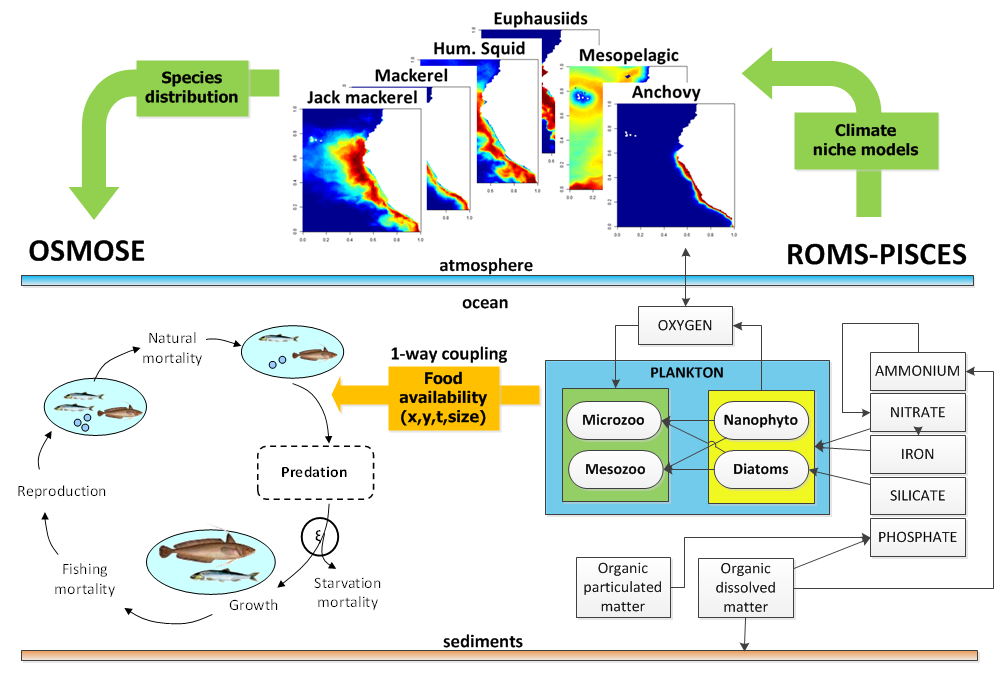
\includegraphics[width=0.9\textwidth]{figures/E2E_osmose}
\caption{Schematic representation of the key processes linking OSMOSE and ROMS-PISCES.}
\label{figure-E2E}
\end{figure}

Once the different pieces of the E2E model were assembled, an essential step consisted in calibrating the model using time series of data, and to do this rigorously, a specific algorithm had to be developed for the specific case of stochastic individual-based models (IBM). We significantly improved the convergence rate of a previous version of an evolutionary algorithm (Duboz et al. 2010) dedicated to OSMOSE calibration and we made the algorithm compatible with well-documented objective functions. In many respects, the calibration of ecosystem models such as OSMOSE is a complex task. In particular, the dynamics represented in ecosystem models allow species-specific parameters to have an impact on one another through ecological interactions, which results in highly correlated parameters, while additionally, critical information and observations on non-commercial species can be missing or poor. Furthermore, the high number of parameters and the long duration of the simulations can be an obstacle to calibrate a model. These diverse reasons hampered the development of flexible and generic enough calibration algorithms and methodologies for ecosystem models, and only sparse documentation has been produced on fitting complex models (Bolker et al. 2013). There are some dedicated tools for non-linear parameter estimation, AD Model Builder (ADMB, Fournier et al. 2012) being one of the most robust and fast (Bolker et al. 2013). Among other advantages, ADMB provides support for calibration in multiple phases (Nash and Walker-Smith 1987), which can be of great interest for the calibration of complex ecosystem models. It also provides support for constraining optimization, which can be helpful for regularizing hard optimization problems (Bolker et al. 2013). However, the model and the objective function itself need to be coded in C++ (using the ADMB scripting), which can be an obstacle for calibrating complex models already implemented in other languages (e.g. Java, Fortran). In addition, as ADMB is based on automatic differentiation, which allows to provide accurate estimates of derivatives (Griewank and Corliss 1992), the tool is not suited for stochastic models for which derivatives cannot be computed, like Individual Based Models (IBM). Parameter estimation methods have been developed for stochastic non-linear models for which the probability of state transitions or the master equation can be written (Ionides et al. 2006, Newman et al. 2009, Ross et al. 2009, Walker et al. 2006). However, many IBMs can only be simulated numerically and are too complex for mathematical analysis and explicit parameter estimation (Black and McKane 2012), resulting in more attention being given to the exploration of model behavior than to a rigorous confrontation with data. As alternative methods, meta-heuristic algorithms have been developed (Cropper and Anderson 2004, Poovathingal and Gunawan 2010, Duboz et at. 2010, Tashkova et al. 2012, Travers-Trolet et al. 2013), and have in some cases shown better performance than derivative-based optimization methods (Tashkova et al. 2012). However, the scientific community lacks generic and flexible enough tools for the calibration of different types of ecological models with different degrees of complexity. In this respect, a major part of this thesis has been dedicated to the conceptual and technical development of calibrar, an R package (R Development Core Team 2014) for the calibration of complex models, in particular stochastic ones. The main features of this software are shown in Figure 2.


\begin{figure}[t]
\centering 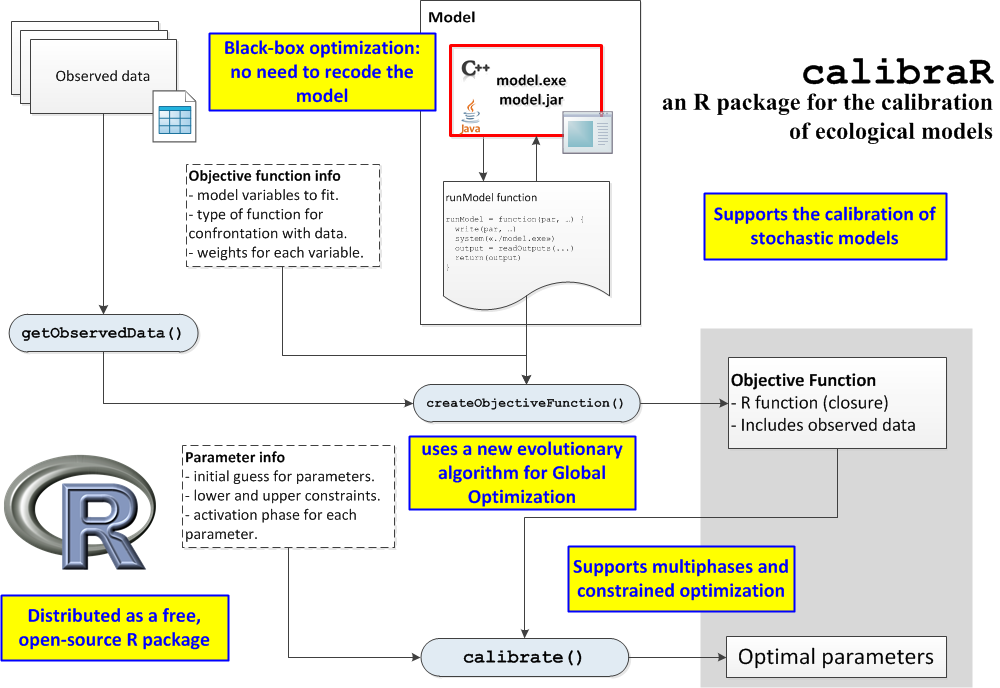
\includegraphics[width=0.9\textwidth]{figures/calibraR}
\caption{Diagram representing the functioning of the calibrar package. The grey area groups the outputs produced for the package (the objective function and the optimal parameters of the model). Rectangles with broken border lines show user inputs which are needed to configure the calibration. Rounded rectangles show main package functions.}
\label{figure-calibrar}
\end{figure}

Given that the calibration of complex ecosystem models requires a lot of data and potentially involves a high number of parameters to estimate, common practice in the field has been to i) reduce the number of parameters to estimate by using estimates provided by other models (Marzloff et al. 2009, Lehuta et al. 2010) or available for similar species or ecosystems (Bundy 2005, Ruiz and Wolff 2011), ii) use other models outputs as data to calibrate the model (Mackinson and Daskalov 2007), or both (Shannon et al. 2003, Guénette et al. 2008, Friska et al. 2011, Travers-Trolet et al. 2013). These different strategies allow to calibrate complex models while attempting to synthesize the maximum of available information. However, as the parameters or outputs used rely on different model assumptions, they may lead to the fitting of artificial parameter values or to inconsistent behavior of the model by trying to reproduce other models' dynamics. Additionally, ecosystem models can require more information to be built, information which may not normally be available (e.g distribution maps for all species). This lack of information is particularly true for non-commercial species or when information required is outside the Economic Exclusive Zone of the countries involved. This situation can limit the development of ecosystem models to areas rich in data. Additional issues can however be raised even in data-rich situations, since the reconstruction of valid spatial information to drive the models is not straightforward.

All these challenges were addressed in this thesis, with the objective to build an end-to-end (E2E) model of the HCE in order to investigate the impacts of environmental variability and fishing scenarios on the management of fishery resources. In the process, the HCE proved to be an ideal model case study to address these issues, as it is a well-studied ecosystem with long time-series of data for species at multiple trophic levels. The main outcomes of this thesis are presented in three chapters and some general conclusions and perspectives are finally drawn to pave the way for future work.

In Chapter 1, we describe the development of an end-to-end model of the Northern Humboldt Current Ecosystem, by coupling ROMS-PISCES and OSMOSE models. We particularly deal with the incorporation of the impact of the interannual variability of the environment and fishing as part of the process of constructing our E2E model. One of the main interannual forcing in OSMOSE is the spatial distribution of fish and other modelled species that we incorporated by building ecological niche models. These models were used to produce monthly maps of spatial distribution for all the species included in our model. For the validation of these niche models, typically based on the classification or regression of binary presence/absence data against several environmental or geographical variables, the confusion matrix and the statistical metrics associated to it are normally used. However, when considering the prediction of the habitat against time, the variability in the spatial distribution of the habitat can be summarized and validated using the emerging patterns from the shape of this distribution. To illustrate this approach, we used jack mackerel (\emph{Trachurus murphyi}) spatial distribution results. The potential habitat was predicted over the study period with monthly resolution, and the model was validated using quantitative and qualitative information of the system compared with i) one dimensional profiles inside the scientific survey area (latitudinal and off-shore distributions) and, ii) time series of the center of gravity of the spatial distribution, modes, quantiles and extremes of the profiles (Manuscript 1: Oliveros et al. in prep). 

In Chapter 2 we present an optimization method that we developed for the calibration of stochastic models, OSMOSE in particular (Manuscript 2: Oliveros and Shin, in review). The calibration algorithm is an Evolutionary Strategy (Beyer and Schwefel 2002) and its implementation as well the tools related to the calibration have been implemented in a package, \texttt{calibrar}, written in R (R Development Core Team 2014). The \texttt{calibrar} package is designed for the optimization of “black-box” functions (Jones et al. 1998), where analytical information about the function to be optimized and the model source code are assumed to be unavailable or impractical to modify (Rios and Sahinidis 2013). Our approach is hence “non-intrusive”, making the model interact with the optimizer, i.e. the \texttt{calibrar} package, in two ways: i) receiving a set of parameters to run, and ii) providing the model outputs to be confronted with the observed data. \texttt{calibrar}also helps in the construction of the objective function to be optimized in order to estimate model parameters (Figure \ref{figure-calibrar}).

In Chapter 3 we propose an approach to deal with the calibration of ecosystem models, and we illustrate it with the end-to-end (E2E) ecosystem model ROMS-PISCES-OSMOSE of the Northern Humboldt Current Ecosystem. Here, we highlight some issues related to the confrontation of complex ecosystem models to data and propose a methodology for a sequential multi-phases calibration of ecosystem models (Manuscript 3: Oliveros et al. in review). We first discuss two criteria to classify the parameters of a model: the model dependency and the time variability of the parameters. Then, these criteria and the availability of approximate initial estimates are used as decision rules to determine which parameters need to be estimated, and their precedence order in the sequential calibration process. The \texttt{calibrar}R package and a likelihood approach are used to fit  monthly time series data of landings, abundance indices and catch at length distributions from 1992 to 2008. 

Finally, we conclude with some perspectives brought out by our work, and particularly on how ecosystem models can be used in the context of the Ecosystem Approach to Fisheries to complement the assessment and recommendations based on single-species models for fishery management.

\section*{References}

Alheit J., Ñiquen M., 2004. Regime shifts in the Humboldt Current ecosystem. Progress in Oceanography 60:201–222.

Aumont, O. E. Maier-Reimer, S. Blain and P. Monfray. 2003. An ecosystem model of the global ocean including Fe, Si, P colimitations. Global Biogeochemical Cycles, (17) 1060.

Bakun, A. and K. Broad., 2003. Environmental loopholes and fish population dynamics: comparative pattern recognition with focus on El Niño effects in the Pacific. Fisheries Oceanography. 12(4/5):458-473.

Beyer, H.-G. and Schwefel, H.-P., 2002. Evolution strategies: a comprehensive introduction, Natural Computing 1:3-52.

Black, A.J. andMcKane, A.J., 2012. Stochastic formulation of ecological models and their applications. Trend in Ecology and Evolution 27(6):337-345. DOI: http://dx.doi.org/10.1016/j.tree.2012.01.014

Bartell S.M., 2003. Effective use of ecological modeling in management: The toolkit concept. In Dale V (editor).Ecological modeling for resource management, Springer Verlag.

Bolker B.M., Gardner B., Maunder M., Berg C.W. , Brooks M., Comita L., Crone E., Cubaynes S., Davies T., de Valpine P., Ford J., Gimenez O., Kéry M., Kim E.J., Lennert-Cody C., Magnusson A., Martell S., Nash J., Nielsen A., Regetz J., Skaug H., Zipkin E., 2013. Strategies for fitting nonlinear ecological models in R, AD Model Builder, and BUGS. Methods in Ecology and Evolution 4: 501–512.

Bundy A., 2005.  Structure and functioning of the eastern Scotian Shelf ecosystem before and after the collapse of ground fish stocks in the early 1990s. Canadian Journal of Fisheries And Aquatic Sciences 62:1453-1473.

Chavez F. P., A. Bertrand, R. Guevara-Carrasco, P. Soler and J. Csirke. 2008. The northern Humboldt Current System: Brief history, present status and a view towards the future. Progress in Oceanography 79:95-105.

Colas F., X. Capet, J.C. McWilliams and A. Shchepetkin. 2008. 1997-1998 El Niño off Peru: A numerical study. Progress in Oceanography 79:138-155. 

Cropper, W.P. Jr. and Anderson, P.J., 2004. Population dynamics of a tropical palm: use of a genetic algorithm for inverse parameter estimation. Ecological Modelling 177: 119–127.

Cury PM, Shin Y-J, Planque B, Durant JM, Fromentin J-M, Kramer-Schadt S, Stenseth NC, Travers M and Grimm V (2008) Ecosystem oceanography for global change in fisheries. Trends in Ecology and Evolution 23:338-346

Duboz, R., Versmisse, D., Travers, M., Ramat, E. and Shin, Y.-J., 2010. Application of an evolutionary algorithm to the inverse parameter estimation of an individual-based model. Ecological Modelling 221(5):840-849.

Echevin V., O. Aumont, J. Ledesma, G. Flores. 2008. The seasonal cycle of surface chlorophyll in the Peruvian upwelling system: A modelling study. Progress in Oceanography 79:167-176.

Echevin V., Goubanova K., Dewitte B., Belmadani A., 2012. Sensitivity of the Humboldt Current system to global warming: a downscaling experiment of the IPSL-CM4 model, Climate Dynamics. doi:10.1007/s00382-011-1085-2.

Fournier D.A., Skaug H.J., Ancheta J., Ianelli J., Magnusson A., Maunder M.N., Nielsen A., Sibert J., 2012. AD Model Builder: using automatic differentiation for statistical inference of highly parameterized complex nonlinear models. Optimization Methods and Software, 27:2, 233-249, DOI: 10.1080/10556788.2011.597854.

Friska M.G., Miller T.J., Latour R.J., Martell S.J.D., 2011. Assessing biomass gains from marsh restoration in Delaware Bay using Ecopath with Ecosim. Ecological Modelling 222:190–200.

Garcia, S.M.; Zerbi, A.; Aliaume, C.; Do Chi, T.; Lasserre, G. 2003. The ecosystem approach to fisheries. Issues, terminology, principles, institutional foundations, implementation and outlook. FAO Fisheries Technical Paper. No. 443. Rome, FAO. 71 p.

Griewank, A. and Corliss, G.F., 1992. Automatic Differentiation of Algorithms: Theory, Implementation, and Application. SIAM, Philadelphia, PA, USA.

Guénette S., Christensen V., Pauly D., 2008. Trophic modelling of the Peruvian upwelling ecosystem: Towards reconciliation of multiple datasets. Progress in Oceanography 79: 326–335.

Ionides, E. L., Breto, C. and King, A.A., 2006. Inference for nonlinear dynamical systems. PNAS 103(49): 18438–18443.

Jones, G. (1998) Genetic and evolutionary algorithms. In Encyclopedia of Computational Chemistry (Schleyer, P .v.R. et al., eds), pp. 1127–1136, John Wiley \& Sons.

Jorgensen S.E. and FathB.D., 2011. Fundamentals of Ecological Modelling: Applications in Environmental Management and Research. Fourth Edition. Elsevier. 350pp.

Lehuta S., Petitgas P., Mahévas S., Huret M., Vermard Y., Uriarte A.,  Record N.R.,  2013. Selection  and  validation  of  a  complex  fishery  model  using  an  uncertainty hierarchy. Fisheries  Research  143:57–  66.

Mackinson S., and Daskalov G., 2007. An ecosystem model of the North Sea for use in research supporting the ecosystem approach to fisheries management: description and parameterisation [online]. (CEFAS, Lowestoft.) Available from www.cefas.co.uk/publications/techrep/tech142.pdf. 

Marzloff M., Shin Y.-J., Tam J., Travers M., Bertrand A., 2009. Trophic structure of the Peruvian marine ecosystem in 2000–2006: Insights on the effects of management scenarios for the hake fishery using the IBM trophic model Osmose. Journal of Marine Systems 75: 290-304.

Nash J.C. and Walker-Smith M., 1987. Nonlinear Parameter Estimation: an Integrated System in BASIC. Marcel Dekker, New York. 493pp.

Newman, K.B., Fernández, C., Thomas, L. and Buckland, S.T., 2009. Monte Carlo Inference for State–Space Models of Wild Animal Populations. Biometrics 65, 572–583.

Ñiquen M., Bouchon M., Ulloa D., Medina A., 2013. Analysis of the Jack mackerel Trachurus murphyi fishery in Peru. Rev. Peru. Biol. 20(1):097-106. 

Penven, P., V. Echevin, J. Pasapera, F. Colas, J. Tam. 2005. Average circulation, seasonal cycle, and mesoscale dynamics of the Peru Current System: A modeling approach. J. Geophys. Res., Vol. 110, No. C10, C1002110.1029/2005JC002945.

Poovathingal, S.K andGunawan, R., 2010. Global parameter estimation methods for stochastic biochemical systems, BMC Bioinformatics 11:414. 

R Core Team (2014) R: A language and environment for statistical computing. R Foundation for Statistical Computing, Vienna, Austria. URL http://www.R-project.org/.

Rios, L.M. \& Sahinidis, N.V. (2013) Derivative-free optimization: a review of algorithms and comparison of software implementations. Journal of Global Optimization 56:1247–1293.

Ross, J.V., Pagendam, D.E. andPollet P.K., 2009. On parameter estimation in population models II: Multi-dimensional processes and transient dynamics. Theoretical Population Biology 75: 123132.

Ruiz D.J, Wolff M., 2011. The Bolivar Channel Ecosystem of the Galapagos Marine Reserve: Energy flow structure and role of keystone groups. Journal of Sea Research 66 123–134.

Shannon L.J., Moloney C.L., Jarre A., Field J.G., 2003. Trophic flows in the southern Benguela during the 1980s and 1990s. Journal of Marine Systems 39:83 – 116.

Shchepetkin, A. F., and J. C. McWilliams, 2003. A method for computing horizontal pressure-gradient force in an ocean model with a nonaligned vertical coordinate, J. Geophys. Res.,108 (C3), 3090, doi:10.1029/2001JC001047.

Shchepetkin, A. F., and J. C. McWilliams, 2005. The regional oceanic modeling system (ROMS): A split-explicit, free-surface, topography-following-coordinate oceanic model, Ocean Modell., 9 , 347–404.

Shin Y.-J., P. Cury. 2001. Exploring fish community dynamics through size-dependent trophic interactions using a spatialized individual-based model. Aquatic Living Resources, 14(2): 65-80.

Shin Y.-J., P. Cury, 2004. Using an individual-based model of fish assemblages to study the response of size spectra to changes in fishing. Canadian Journal of Fisheries and Aquatic Sciences, 61: 414-431.

Tashkova, K., Silc, J., Atanasova, N. andDzeroski, S., 2012. Parameter estimation in a nonlinear dynamic model of an aquatic ecosystem with meta-heuristic optimization. Ecological Modelling 226: 36– 61.

Travers-Trolet, M., Shin, Y.-J. and Field, J.G., 2013. An end-to-end coupled model ROMS-N2P2Z2D2-OSMOSE of the southern Benguelafoodweb: parameterisation, calibration and pattern-oriented validation, African Journal of Marine Science, 36:1, 11-29,  DOI:10.2989/1814232X.2014.883326

United Nations. 2004. Overfishing: a threat to marine biodiversity. “Ten Stories the World Should Know More About.” http://www.un.org/events/tenstories/

Walker, D.M., Pérez-Barbería, F.J. and Marion, G., 2006. Stochastic modelling of ecological processes using hybrid Gibbs samplers. Ecological Modelling 198:40-52.




\cleardoublepage

\chapter{Incorporating the impact of the interannual variability of the environment}
\label{interannual} 
\chaptermark{Incorporating the impact of the interannual variability}
\thispagestyle{empty}%
The Humboldt Current Ecosystem (HCE) is characterized by a high environmental variability, influencing the distribution and abundance of the main fish stocks. The objective of this thesis was to develop an integrated and multidisciplinary end-to-end (E2E) model of the Northern HCE, including the explicit dynamics of the physical environment, the primary and secondary production, as well as the exploited fish communities. For this purpose, the OSMOSE model was selected to represent the High Trophic Level (HTL) community and an existing application of the ROMS-PISCES hydrodynamic and biogeochemical model for the HCE (Echevin et al. 2012) was selected to represent explicitly the seasonal and interannual forcing from the Low Trophic Level (LTL) community and the physical environment. The interannual effect of fishing was introduced in the OSMOSE model as time series of fishing mortality, which were estimated during the calibration process in order to properly fit the landings data. In the first section of this chapter we start by describing the OSMOSE component model that we had to fully parameterize to represent the dynamics of the HTL community of the NHCE, then briefly describe the ROMS-PISCES model available for the HCE and how its outputs were used to force the OSMOSE model, while in the last section we show how we constructed and validated the spatial maps of the distribution of the modeled species, also used to force OSMOSE. The impact of the interannual variability of fishing and how it is modeled are described in chapter 3.

\section{Modeling the HTL dynamics: OSMOSE}


In OSMOSE, the basic unit of simulation is the ``school'', a group of individuals of the same species sharing the same properties and history in terms of spatial position, length and age. The state of each school in the system can be described by a vector $S = (s, x, y, N, L, A)$, where $s$ is the species the school belongs to, $(x,y)$ is the position of the school (longitude, latitude), $N$ is the number of individuals in the school (abundance), $L$ is the body length of the individuals and $A$ is its age. At any time, the state of the system can be described by the state of all living schools  ($N>0$).
There are three main processes controlling the dynamic of a school: mortality, somatic growth and spatial movement. The core of the first two processes relies in very simple survival and growth assumptions:

\begin{eqnarray}
N(t+1) & = & e^{-Z}N(t)\\
L(t+1) & = & L(t) + G
\end{eqnarray}


In OSMOSE, the total mortality ($Z$) and growth in length ($G$) during a time step are functions of the state of the school itself and that of all other schools in a defined neighbourhood given by the discretization of the spatial domain. This means growth and mortality are function of the state of all schools which are present in the same cell of the grid at the same time. In the OSMOSE version considered in this work, the functions defining mortality and growth are deterministic, while the main source of stochasticity is in the movement process. 

After one time step, each school can move to an adjacent cell of the grid or remain in the same position in a uniform random way. Additionally, the model is forced by species-specific spatial distribution maps. At any time, each school can be assigned to a unique map, while this map can change during the simulation according to age or time-specific criteria (e.g. seasonal maps, different maps for adults or juveniles). When a change in the map for a school occurs, the school is relocated randomly in the new map according to its spatial probability distribution (which can be uniform in the simplest case).

Taken this into account, growth and mortality in OSMOSE depend stochastically on the complex interactions between several schools of different species.
Mortality and growth both depend on the predation process which is length based in OSMOSE. For each species, a school can feed on prey within a limited range of sizes, parameterized by the minimum and maximum ratio between predator and prey sizes. This rule allows each school to ``select'' which other schools it can feed on, considering only the length of the individuals and the co--occurrence in the same cell, so that for most modeled species in the pelagic column, no a priori species-specific trophic relationship is assumed. As a result, the diets, trophic levels and predation mortalities are derived quantities from the model and the size-based predation assumption, and produced as outputs of OSMOSE.

A key parameter linking predation with growth and mortality is the critical predation efficiency threshold $\xi_{max}$, defined as the threshold corresponding to maintenance needs of a fish, and beyond which the food ration can be dedicated to fish growth (Shin and Cury 2001, Shin et al. 2004). This parameter allows correcting the actual growth (no growth below $\xi_{max}$) in the mean length of the school, and adding a starvation mortality $M_\xi$ to the total mortality when predation efficiency is below $\xi_{max}$ (Shin and Cury 2001). 


The size of the fish is modeled by a linear relationship below a critical age or length (fast growth at initial stages, and for which von Bertalanffy growth parameters are usually not well estimated), and beyond that age/size threshold is modeled using the von Bertalanffy model. The actual growth rate (difference in size between two time steps) is calculated on the basis of the von Bertalanffy growth model but taking into account a deviation depending on the predation efficiency at each time step, according to Shin and Cury (2001).


The total mortality for a school is calculated taking into account the food ration needed by co-occurring predator schools (predation mortality), the fishing mortality, the starvation mortality and an additional mortality component $M_0$ representing the mortality due to other processes which are not fully explicit in the model (e.g. due to other predators). The total mortality and its components for each school in the same cell of the grid are solved simultaneously for all species. 

An additional important process leading to the renewal of the population is the reproduction process. Here, the total spawner biomass of each species (aggregated over all schools given a size or age of maturity and sex ratio) leads to an egg production (age 0 abundance). While the recruitment level emerges from the different sources of mortality applied at the subsequent time steps, the initial total egg production is assumed proportional to the spawner biomass, the potential relative fecundity (number of eggs per gram of mature female by unit of time) being the factor of proportionality. These eggs are distributed in a number of new schools proportional to the area of distribution of the species and the expected average biomass of the population for the modeled period. This means that for species with bigger distribution areas, abundance, or both, more new age-0 schools are introduced in the model at each time step. The initial state of the new schools is given by: (i) abundance: the number of eggs after the distribution of the total egg production among all the new schools, (ii) length: the assumed size of the egg for the species, (iii) position: randomly distributed within the age-0 map for the species, and (iv) age 0.

The dynamics of the low trophic level (LTL) species is not explicit in the model, reason why plankton fields (provided by observations or biogeochemical models) are used as forcing variables, representing additional food for planktivorous species or for the smaller species and size classes in OSMOSE. The LTL biomass is available to predation in the same way school biomass is in OSMOSE.

The constants, state variables, parameters, forcings, initial conditions and main derived quantities used in the OSMOSE model are described in Tables \ref{tab:osmose-vars1} and \ref{tab:osmose-vars2}.


\begin{table}
\caption{Description of main quantities used in the OSMOSE model (1).}
\label{tab:osmose-vars1}
\centering \footnotesize 
\begin{tabular}{|p{5cm}|c|c|p{5cm}|}
\hline & Symbol & Units & Remarks\\
\hline \multicolumn{4}{|l|}{1. Constants}\\
\hline Number of low trophic level groups & $N_P$ &&	Species or functional groups from LTL model.\\
\hline Number of species modeled & $N_S$ && Species or functional groups modeled in OSMOSE.\\
\hline Number of age-0 schools & $n^s$ & year$^{-1}$ & Number of new schools per year for species $s$.\\
\hline Number of simulation steps per year	& $N$ &	year$^{-1}$ & \\
\hline Number of simulation years & $T$ & year &  \\
\hline \multicolumn{4}{|l|}{2. State variables}\\	
\hline Number of schools alive & $n^{\#}$ && Schools with positive abundance. \\
\hline Species	& $S$ && $s = 1, \ldots , N_S$\\
\hline Spatial position &	$(x,y)$ & degrees & Position in latitude and longitude.\\
\hline Abundance of the school & $N$ & ind & Number of individuals \\
\hline Average length of individuals of a school & $L$ &cm & \\	
\hline Age of individuals of a school & $A$ & year & \\	
\hline State of a school & $S$ && $S = (s, x, y, N, L, A)$ \\
\hline \multicolumn{4}{|l|}{3. Forcing variables}\\ 
\hline Biomass of plankton from LTL & $B_p(t,x,y)$	& tonnes/km$^2$ & $p = 1, \ldots, N_P$\\
\hline Probability of presence in the habitat & $P_s(t,x,y,a)$ &&	$s = 1, \ldots, N_S$\\
\hline \multicolumn{4}{|l|}{4. Parameters}\\
\hline Critical predation efficiency & $\xi_{max}$ && \\		
\hline Maximum starvation mortality& $M_{\xi,max}^s$ & year$^{-1}$ & \\	
\hline Life history parameters	& $\Phi_s$ && $\Phi_s =~(A_{max}, k, L_{\infty}, t_0, A_{thr}, \newline a, b, l_{egg}, w_{egg}, p_f, L_{50})$, \newline vB equation, length--weight\\
\hline Predation size ratios & $\rho_{s,min}(a,l)$ && $s = 1, \ldots, N_S$\\
& $\rho_{s,max}(a,l)$ && \\
\hline Base natural mortality & $M_s(t,x,y,a,l)$ & year$^{-1}$ & \\	
\hline Fishing mortality &	$F(s,t,x,y,a,l)$ & year$^{-1}$ & \\	
\hline Plankton accessibilities & $\alpha_{p,s}(t)$ && Fraction of plankton group $p$ accessible to predators species $s$ \\
\hline Predation accessibilities & $\alpha_{s,r}(t)$ && Fraction of species group $s$ accessible to predators species $r$ \\
\hline Fecundity & $\varphi^s(t)$ & eggs/tonne/year & \\
\hline Larval mortality & $\lambda^s(t)$ &  month$^{-1}$ & \\	
\hline Inmigration biomass flux & $\psi^s(t)$ & tonnes & \\	
\hline Average length of migratory schools	& $L$ & cm & \\	
\hline Age of migratory schools & $A$ & years & \\	
\hline
\end{tabular} 
\end{table}


\begin{table}
\caption{Description of main quantities used in the OSMOSE model (2).}
\label{tab:osmose-vars2}
\centering \footnotesize 
\begin{tabular}{|p{5cm}|c|c|p{4cm}|}
\hline & Symbol & Units & Remarks\\
\hline \multicolumn{4}{|l|}{5. Derived quantities}\\
\hline Spatial distribution of abundance & $N_s(t, x, y)$ & ind/km$^2$ & $s = 1, \ldots, N_S$ \\
Spatial distribution of biomass & $B_s(t, x, y)$ & tonnes/km$^2$ & \\	
\hline Total abundance of the population &  $N_s(t)$ & ind & \\
Total biomass of the population & $B_s(t)$ & tonnes & \\	
\hline Catch-at-age & $C_s(t, a)$ & ind  & \\
Catch-at-length & $C_s(t, l)$ &&\\
\hline Yield & $Y_s(t, x, y)$ & tonnes/km$^2$ & \\	
\hline Total yield	& $Y_s(t)$ &tonnes & \\	
\hline Predation mortality & $P_{s,r}(t, x, y)$ && Prey $s = 1, \ldots, N_S$ \\
Starvation mortality & $M_\xi(s, t, x, y)$ & year$^{-1}$ & Predator $r = 1, \ldots, N_S$\\
Total mortality	& $Z(s, t, x, y)$ && \\ 
\hline Trophic level & $TL(s,t,x,y,l)$ && \\		
\hline \multicolumn{4}{|l|}{6. Initial conditions}\\
\hline Total biomass & $B_0^s$ & tonnes & \\	
\hline School states & $S_0^i = (s, x, y, l, a)$ && $i = 1, \ldots,n_0^\#$.\\
\hline
\end{tabular} 
\end{table}

\section{Interannual forcing of the plankton: ROMS--PISCES}


ROMS (Regional Oceanic Modeling System, Shchepetkin and McWilliams 2005) is a free surface ocean model that solves the primitive equations of oceandynamics. Widely used by the scientific community in a diverse range of applications in the world (Haidvogel et al 2000, Peliz et al 2003, Di Lorenzo 2003, Dinniman et al. 2003, Budgell 2005, Warner et al. 2005a, 2005b, Wilkin et al. 2005), it has been especially designed to produce realistic simulations of the dynamics of regional systems. 

The PISCES (Pelagic Interaction Scheme for Carbon and Ecosystem Studies) biogeochemical model simulates marine biological productivity and describes biogeochemical cycles of carbon and major nutrients in the ocean (Aumont and Bopp 2006). PISCES assumes that phytoplankton growth depends on external concentration of nutrients and that the main nutrients in the medium follow the Redfield ratio (C:N:P $\sim$ 106:16:1) (Redfield et al 1963). PISCES has 24 state variables, among which are nutrients (Phosphorus, Nitrogen, Silica and Iron), dissolved oxygen, two kinds of detritus (large and small), two classes of zooplankton (microzooplankton and mesozooplankton) and two kinds of phytoplankton (nanophytoplankton and diatoms). Diatoms differ from nanophytoplankton in their requirements in silicates, an increased consumption of iron and higher levels of saturation due to its larger size (Echevin et al. 2008).

\subsection{ROMS--PISCES model setup}

In Peru, there have been several modeling studies of climatological variability (Penven et al. 2005, Montes et al. 2010) and the effects of El Niño 1997-1998 (Colas et al. 2008). 

However, the simulations used in this thesis are the first that investigate a period over 15 years (1992-2008) in an area corresponding to the Southeast Pacific delimited between 100º and 70º W and 10º N to 40º S, covering a larger area to the north than the HCE to reproduce more accurately the equatorial circulation, because changes in the dynamics of equatorial currents (surface and subsurface) would influence directly the dynamics (Montes et al. 2010), richness, oxygenation and productivity (Espinoza-Morriberón 2012) of the waters off Peru. In the present study the PISCES model is coupled to the physical model ROMS, following the approach of Gruber et al. (2006), who coupled ROMS to a simpler biogeochemical model than PISCES. The spatial resolution is 1/6º with 32 sigma vertical levels (which follow the topography of the ocean floor). Atmospheric forcings were constructed from: i) binding of climatological SCOW data (Risien and Chelton 2008) with NCEP anomalies (\url{www.ncep.noaa.gov}) for wind fields and, ii) binding of COADS climatology data (Da Silva et al. 1994) with NCEP anomalies for the heat fluxes and air temperatures. For boundary conditions the outputs of the global simulation of the ORCA2-PISCES physical-biogeochemical coupled model (Aumont and Bopp 2006) were used, and they were forced with NCEP data. For more information about the construction of simulation forcings and boundaries, the reader can refer to Echevin et al. (2012), Cambon et al. (2013) and the webpage of the project ``Peru Ecosystem Projection Scenarios (PEPS)'' (\url{www.locean-ipsl.upmc.fr/PEPS}).

\subsection{Coupling ROMS--PISCES with the OSMOSE model}

The results of this ROMS-PISCES simulation were validated through its ability to represent the climatological and interannual variability from 1992 to 2008 (Romero et al. submitted, Espinoza et al. submitted) of the main physical variables corresponding to the South East Pacific ocean region (temperature, salinity, currents and sea level),the distribution of surface water masses, the depth of the oxygen minimum zone (OMZ), as well as concentrations of nutrients and surface chlorophyll-a.  

The concentration fields of the four groups of plankton modeled in PISCES (nanophytoplankton, diatoms, microzooplankton and mesozooplankton) are used as prey fields forcing the OSMOSE model, where planktivorous fish can have access to the plankton according to the size-based predation rules implemented in the model. Additionally, the depth of the oxygen minimum zone is used as a predictor of the spatial distribution of all the modeled species as described in the next section.

\begin{figure}
\centering
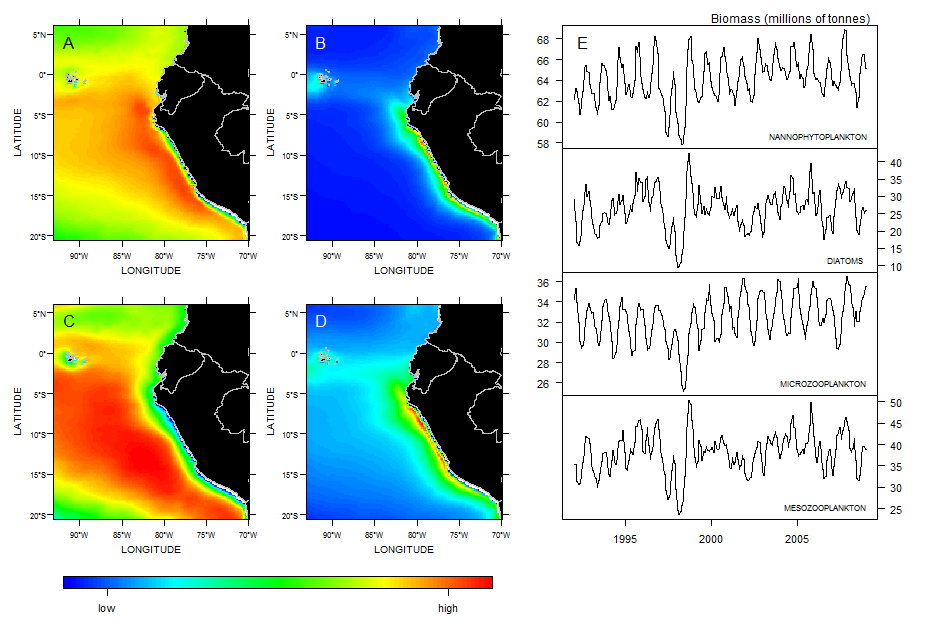
\includegraphics[width=0.95\linewidth]{figures/figuraA1}
\caption{Summary of the LTL biomass simulated by ROMS-PISCES model used as forcing for OSMOSE. Average spatial distribution for nanophytoplankton (A), diatoms (B), microzooplankton (C) and mesozooplankton (D) (red is high, blue is low, following the light visible spectrum). Simulated temporal dynamics of thetotal biomass (millions of tonnes) of the four plankton groups (E) is also shown.}
\label{fig:figureA1}
\end{figure}



\section{Modelling the variability in fish habitat distribution}

In order to model the interannual variability in the distribution of the species included in the NHCE OSMOSE model, several GAM models were constructed. A more detailed description of the model building and validation for Jack mackerel is presented here, highlighting some of the issues we found when constructing time series of maps. The results for other species are shown thereafter.

\subsection[Pattern--oriented validation of habitat distribution models]{Pattern-oriented validation of habitat distribution models}

The following manuscript is in preparation for submission as a short communication to the ICES Journal of Marine Science.

\includepaper{figures/Oliveros_etal-validation_niche_models-for_print.pdf}


\subsection{Prediction of the spatial distribution of modeled fish in the NHCE} 

Similar models and methods as described in the previous subsection for Jack mackerel were applied to the other species explicitly modeled in OSMOSE (macrozooplankton, anchovy, sardine, chub mackerel, mesopelagic fish, red lobster or munida, jumbo squid and the Peruvian hake). The seasonal patterns of the distribution as a summary of these results are shown in the next figures.

\begin{figure}
\centering
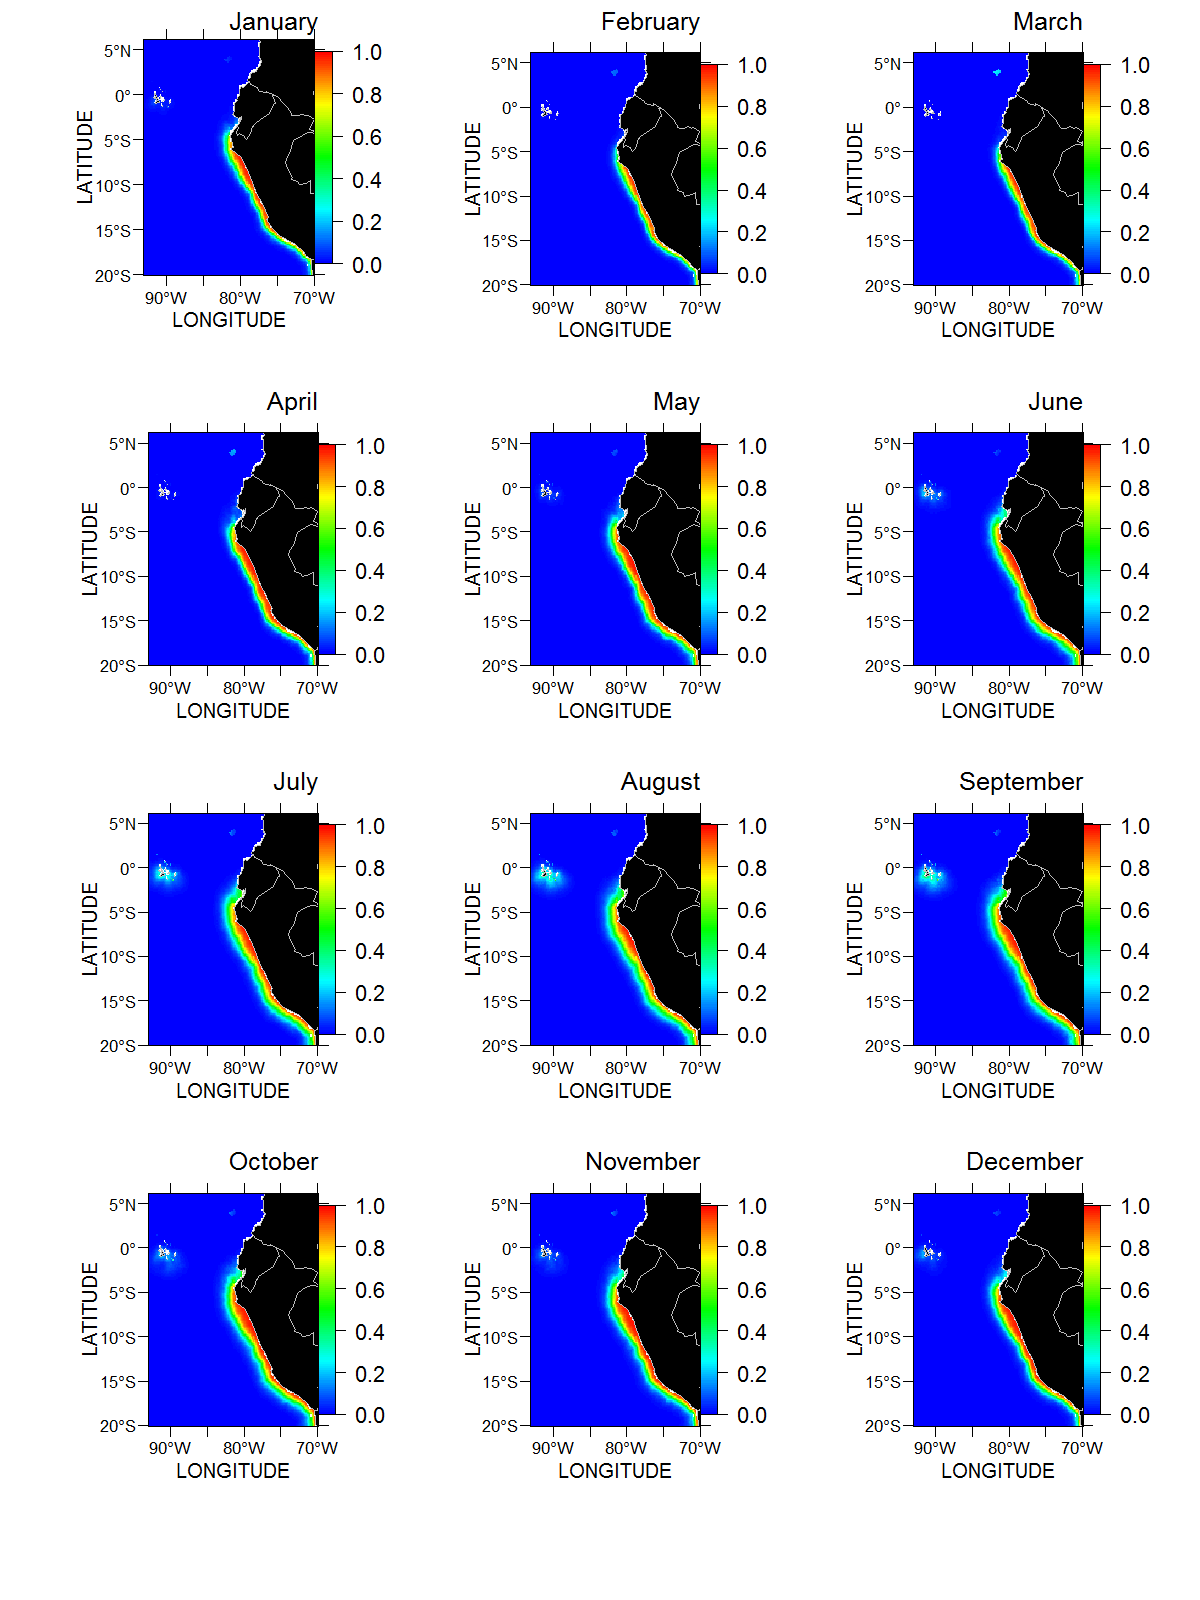
\includegraphics[height=0.8\textheight]{figures/anchovy-climatology}
\caption[Seasonal patterns of the distribution of Peruvian anchovy]{Seasonal patterns of the distribution of Peruvian anchovy as predicted by the species distribution models used to build the interannual maps for the NHCE OSMOSE model.}
\label{fig:anchovy-climatology}
\end{figure}

\begin{figure}
\centering
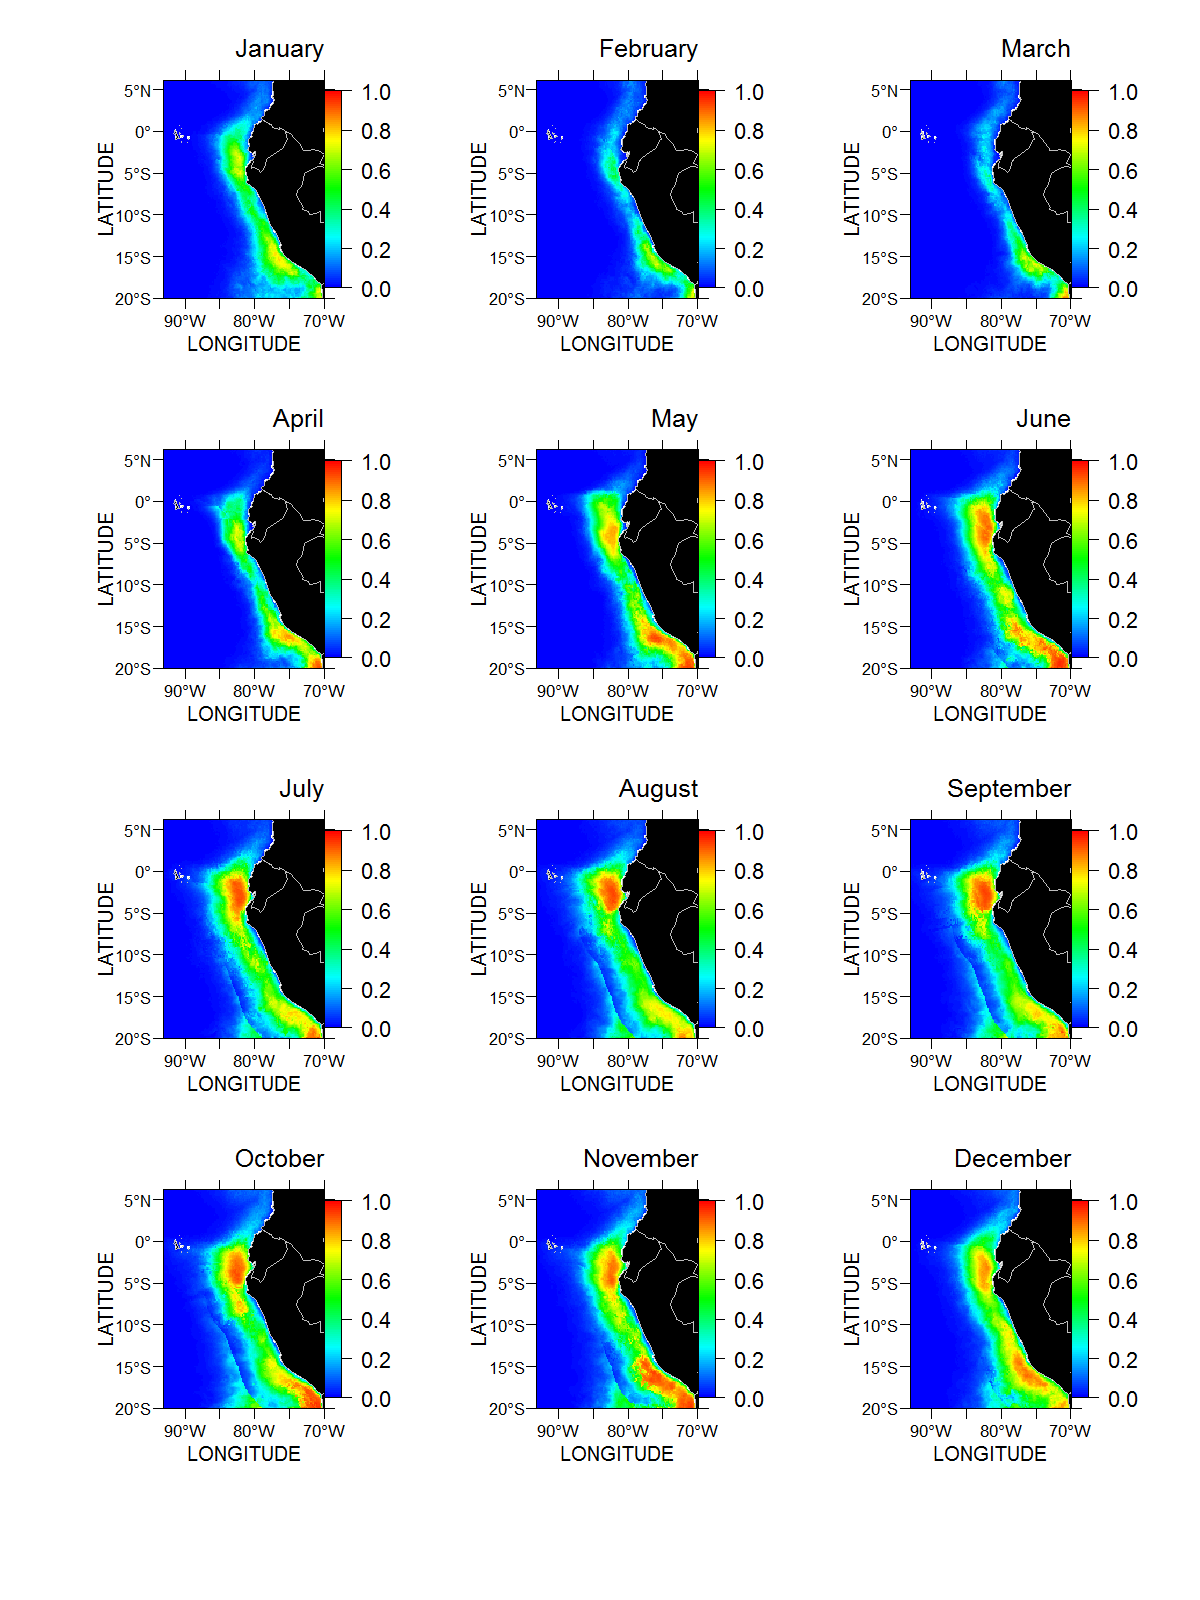
\includegraphics[height=0.8\textheight]{figures/jurel-climatology}
\caption[Seasonal patterns of the distribution of Jack mackerel]{Seasonal patterns of the distribution of Jack mackerel as predicted by the species distribution models used to build the interannual maps for the NHCE OSMOSE model.}
\label{fig:jurel-climatology}
\end{figure}

\begin{figure}
\centering
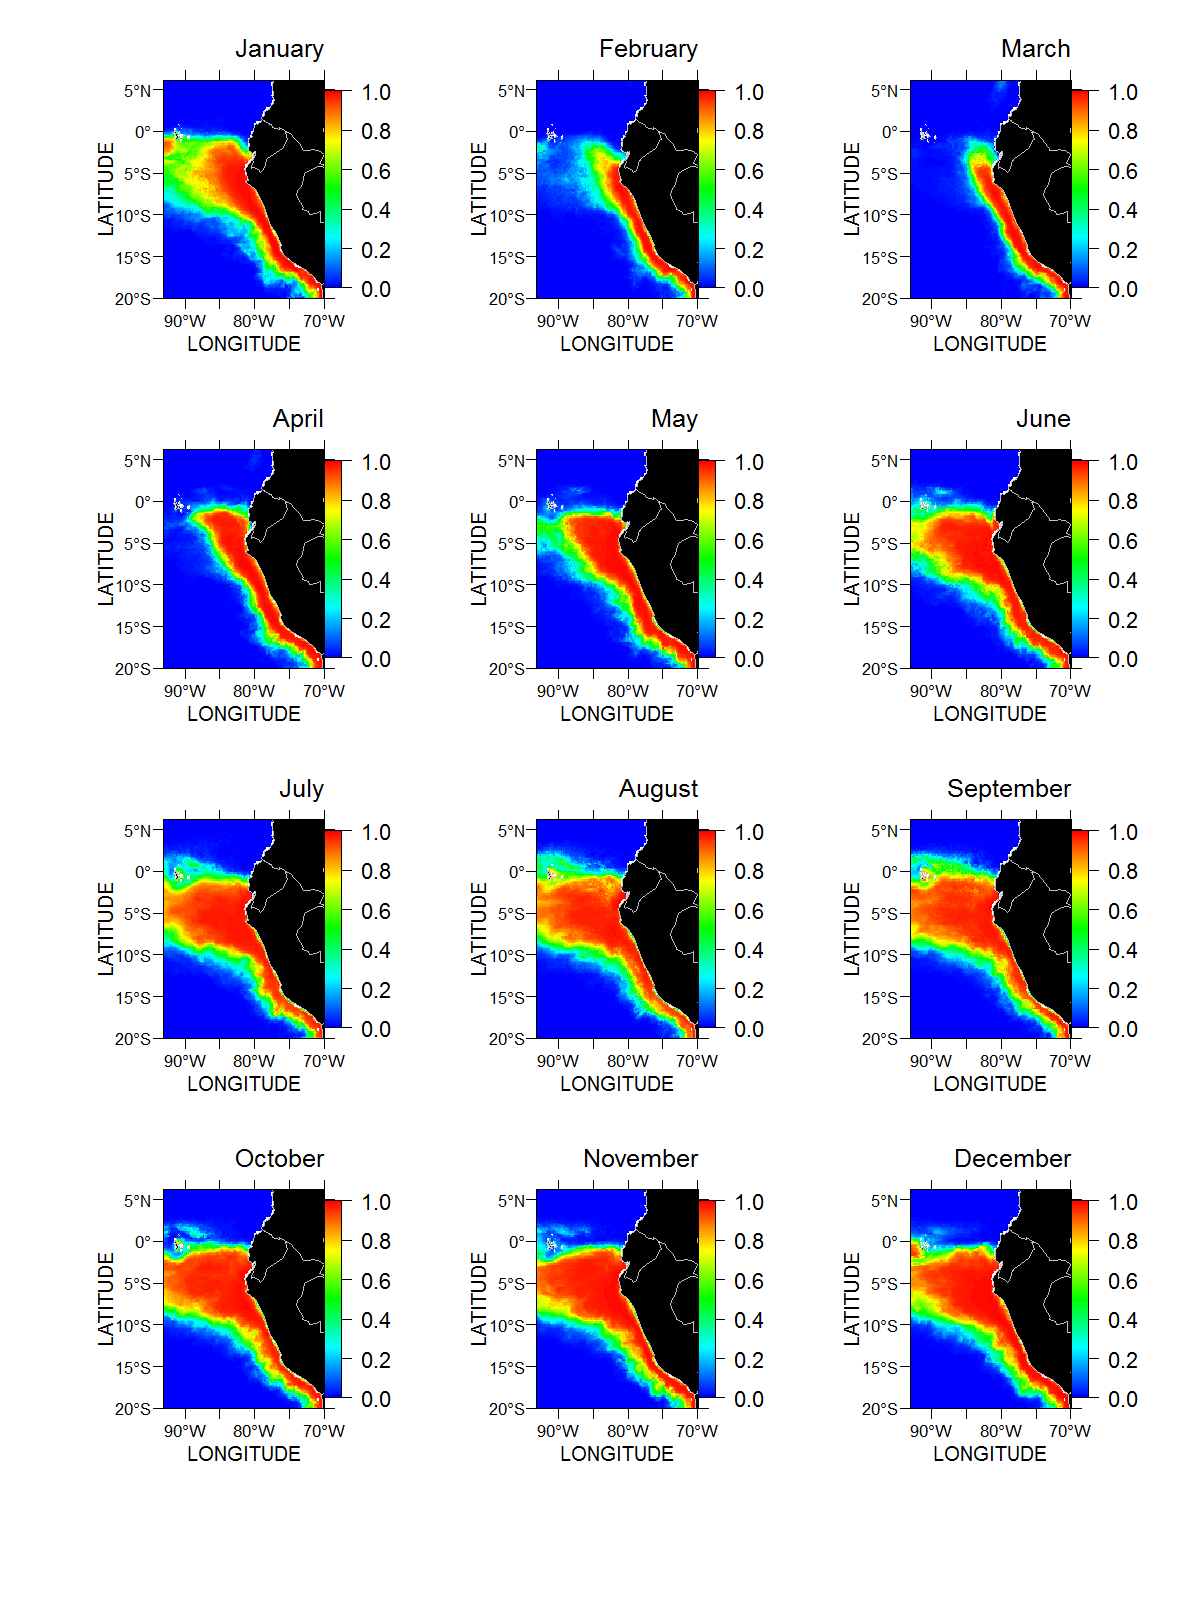
\includegraphics[height=0.8\textheight]{figures/euphausidos-climatology}
\caption[Seasonal patterns of the distribution of Macrozooplankton]{Seasonal patterns of the distribution of macrozooplankton as predicted by the species distribution models used to build the interannual maps for the NHCE OSMOSE model.}
\label{fig:euphausidos-climatology}
\end{figure}

\begin{figure}
\centering
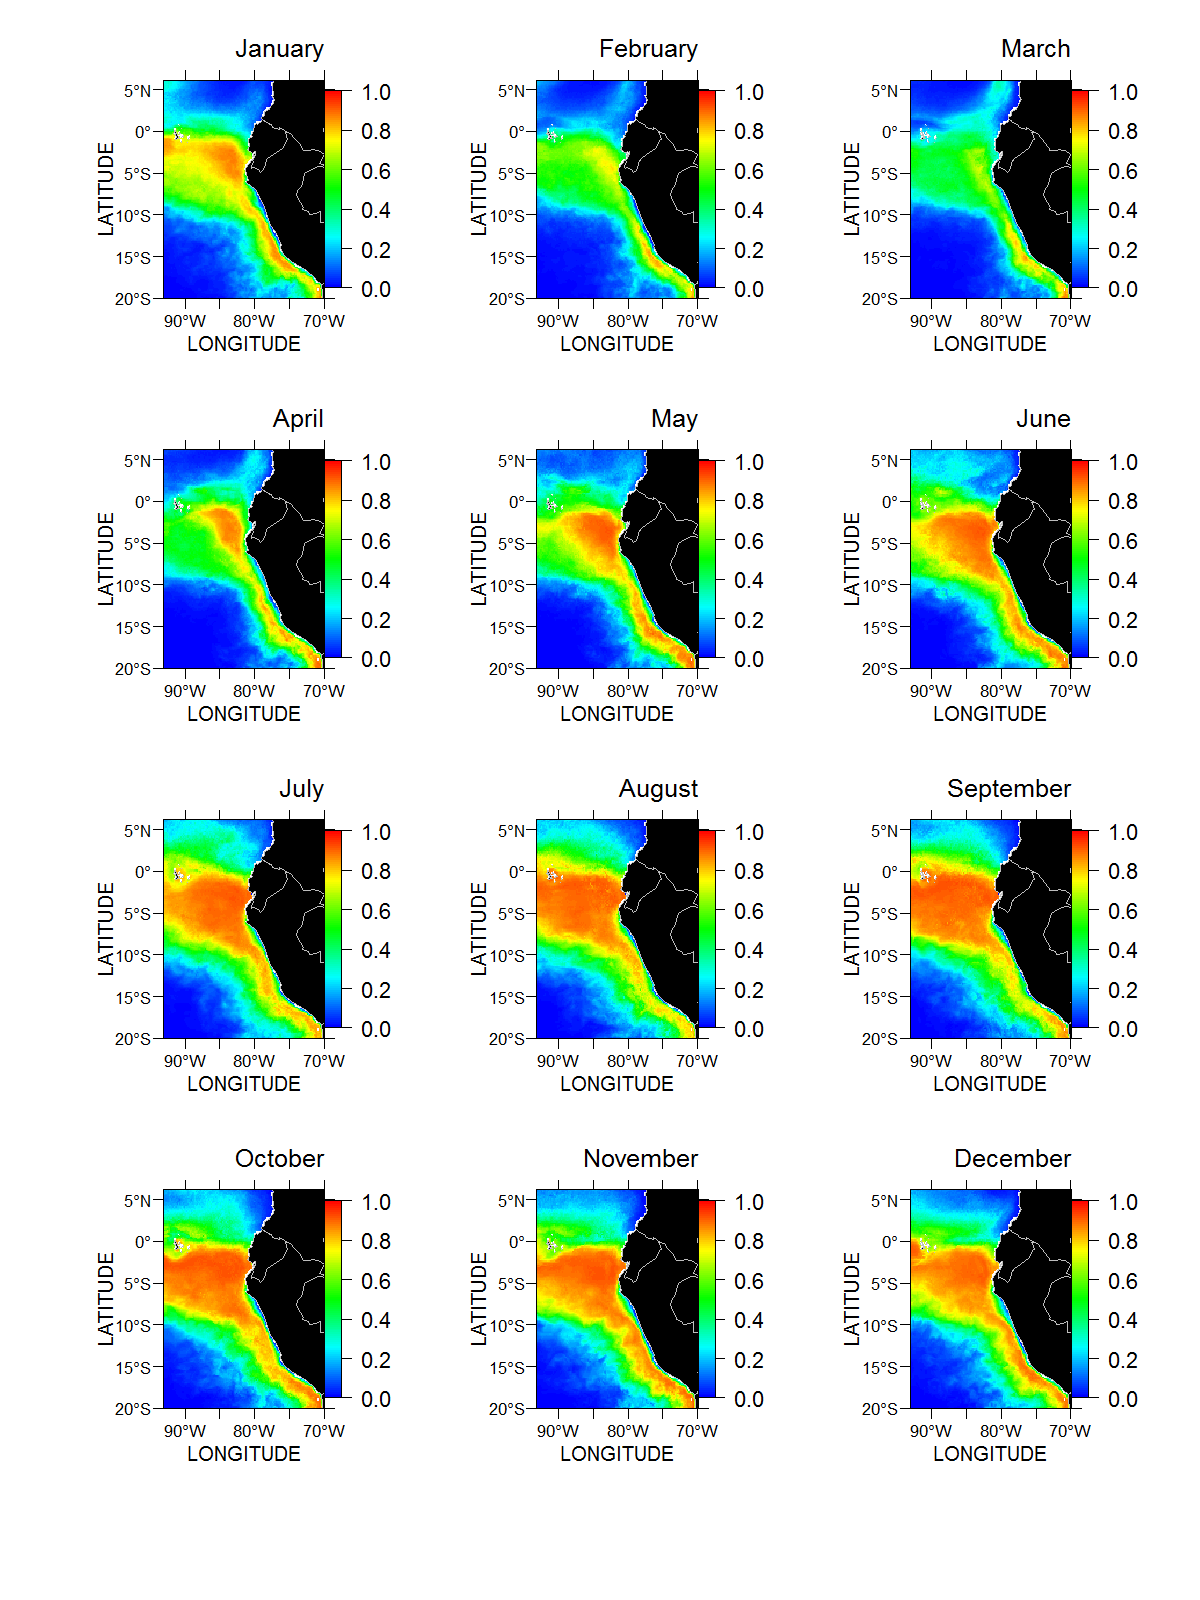
\includegraphics[height=0.8\textheight]{figures/pota-climatology}
\caption[Seasonal patterns of the distribution of Humboldt squid]{Seasonal patterns of the distribution of Humboldt squid as predicted by the species distribution models used to build the interannual maps for the NHCE OSMOSE model.}
\label{fig:pota-climatology}
\end{figure}

\begin{figure}
\centering
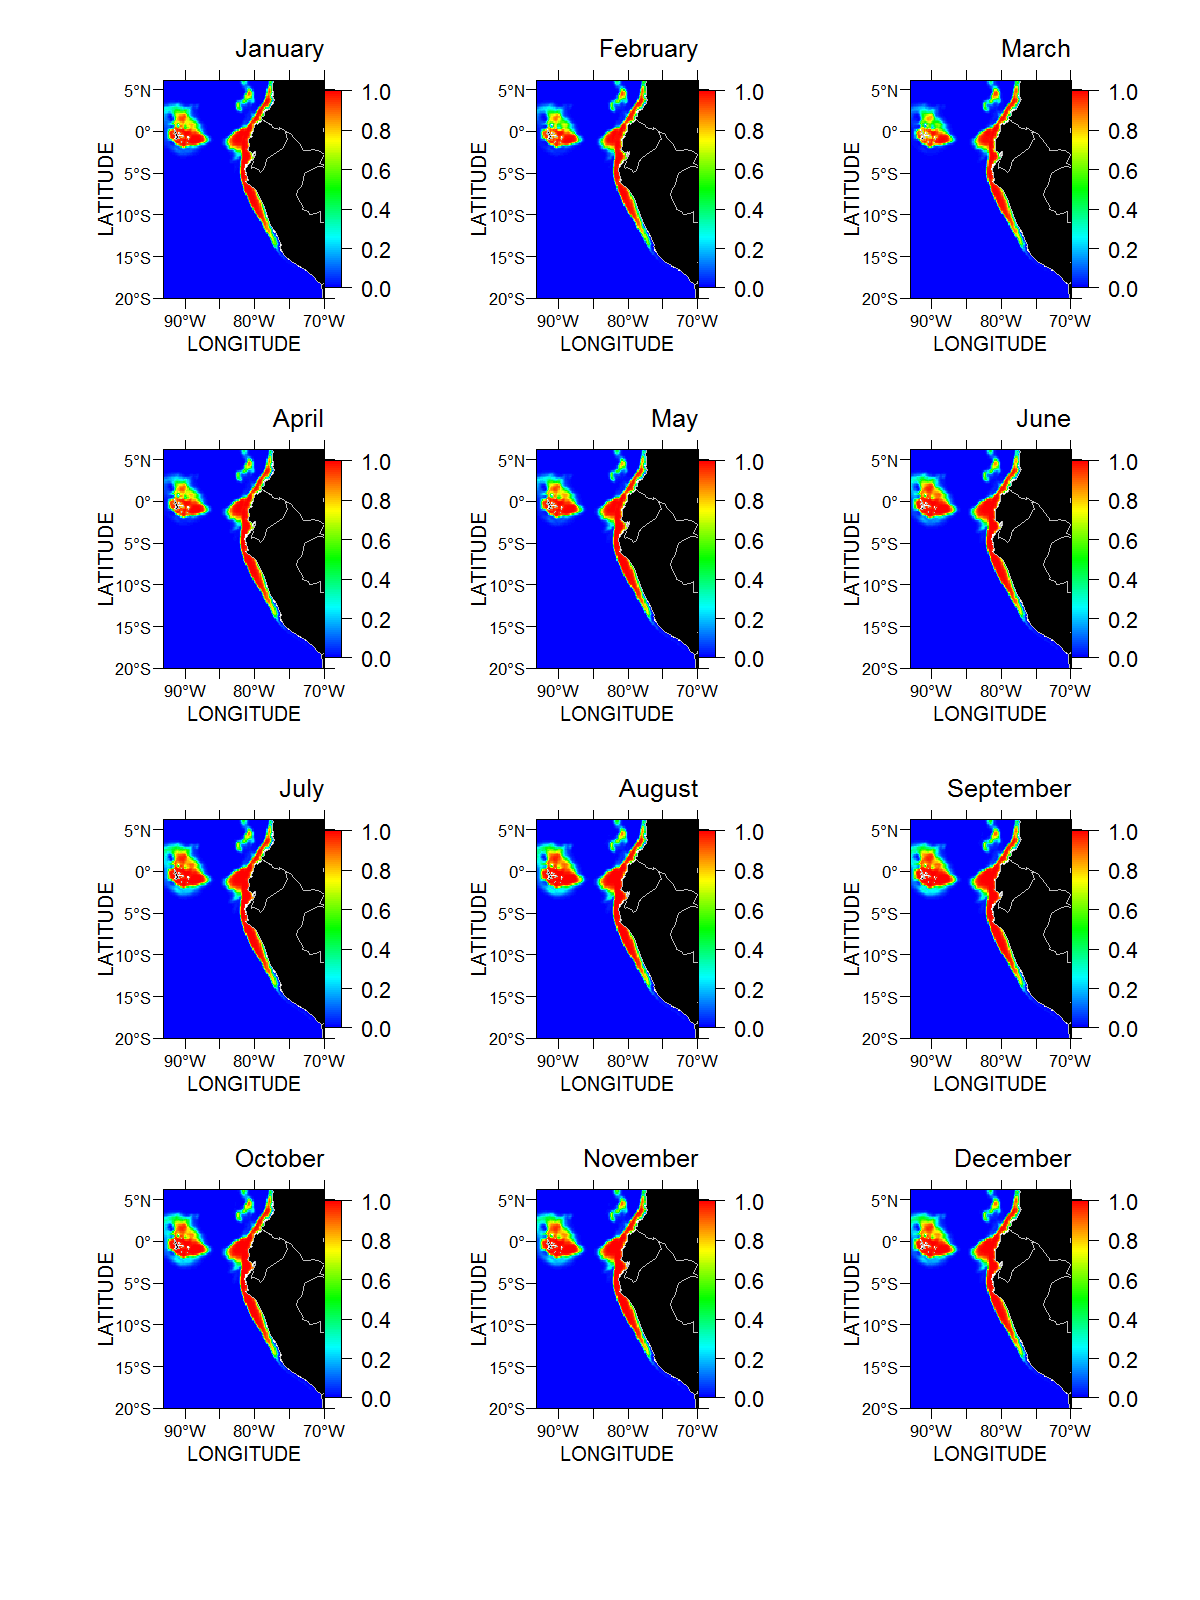
\includegraphics[height=0.8\textheight]{figures/hake-climatology}
\caption[Seasonal patterns of the distribution of Peruvian hake]{Seasonal patterns of the distribution of Peruvian hake as predicted by the species distribution models used to build the interannual maps for the NHCE OSMOSE model.}
\label{fig:hake-climatology}
\end{figure}

\begin{figure}
\centering
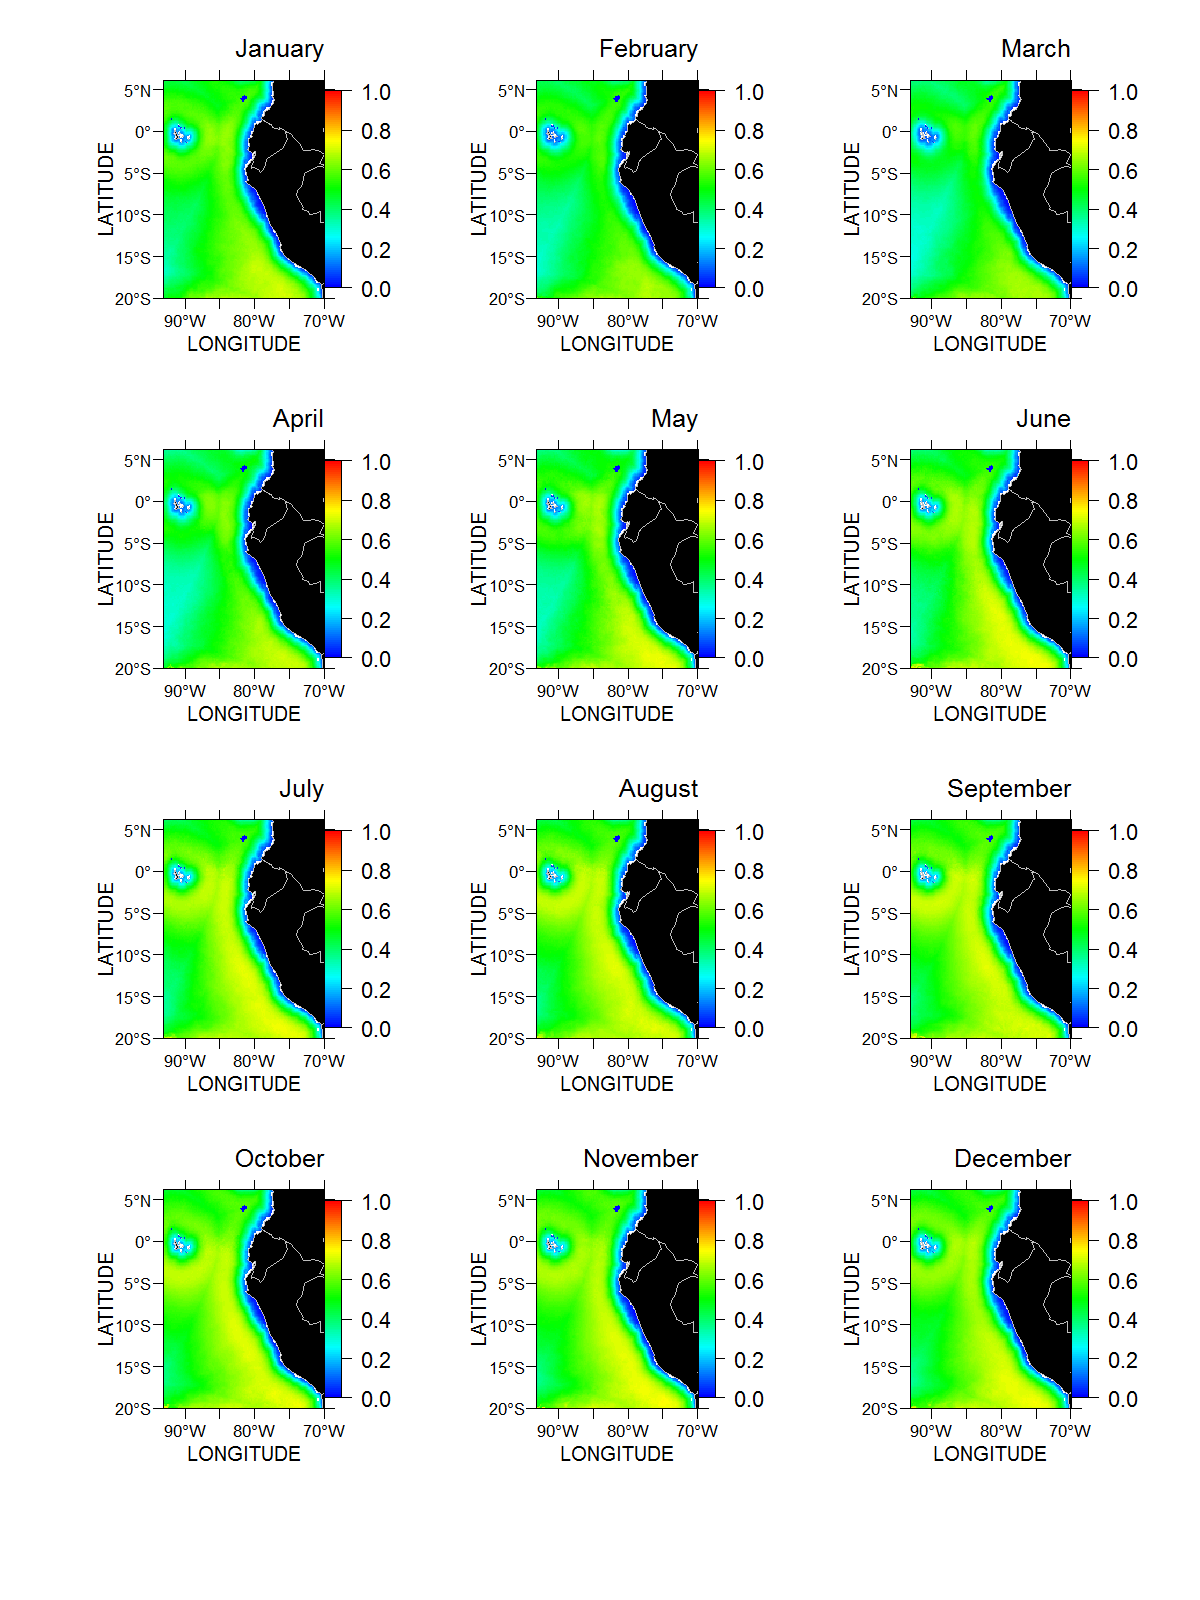
\includegraphics[height=0.8\textheight]{figures/meso-climatology}
\caption[Seasonal patterns of the distribution of mesopelagic fish]{Seasonal patterns of the distribution of mesopelagic fish as predicted by the species distribution models used to build the interannual maps for the NHCE OSMOSE model.}
\label{fig:meso-climatology}
\end{figure}

\begin{figure}
\centering
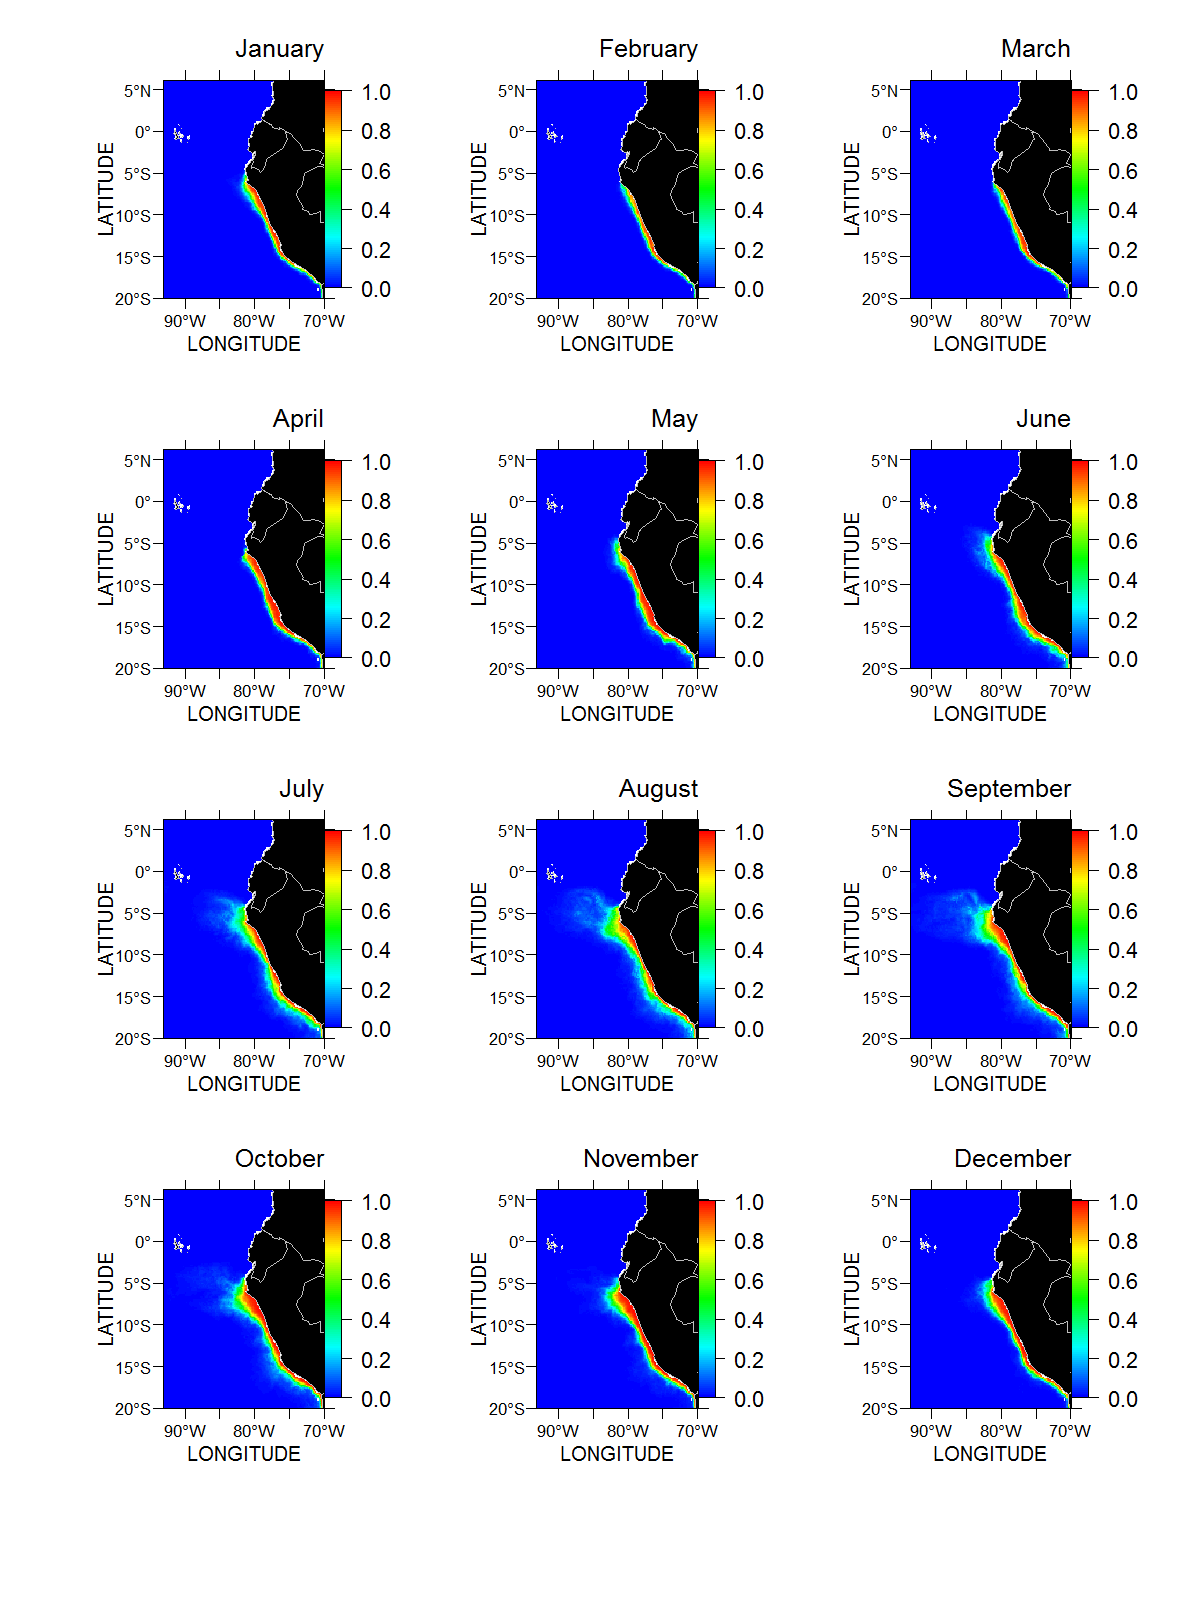
\includegraphics[height=0.8\textheight]{figures/munida-climatology}
\caption[Seasonal patterns of the distribution of Munida]{Seasonal patterns of the distribution of Munida as predicted by the species distribution models used to build the interannual maps for the NHCE OSMOSE model.}
\label{fig:munida-climatology}
\end{figure}

\begin{figure}
\centering
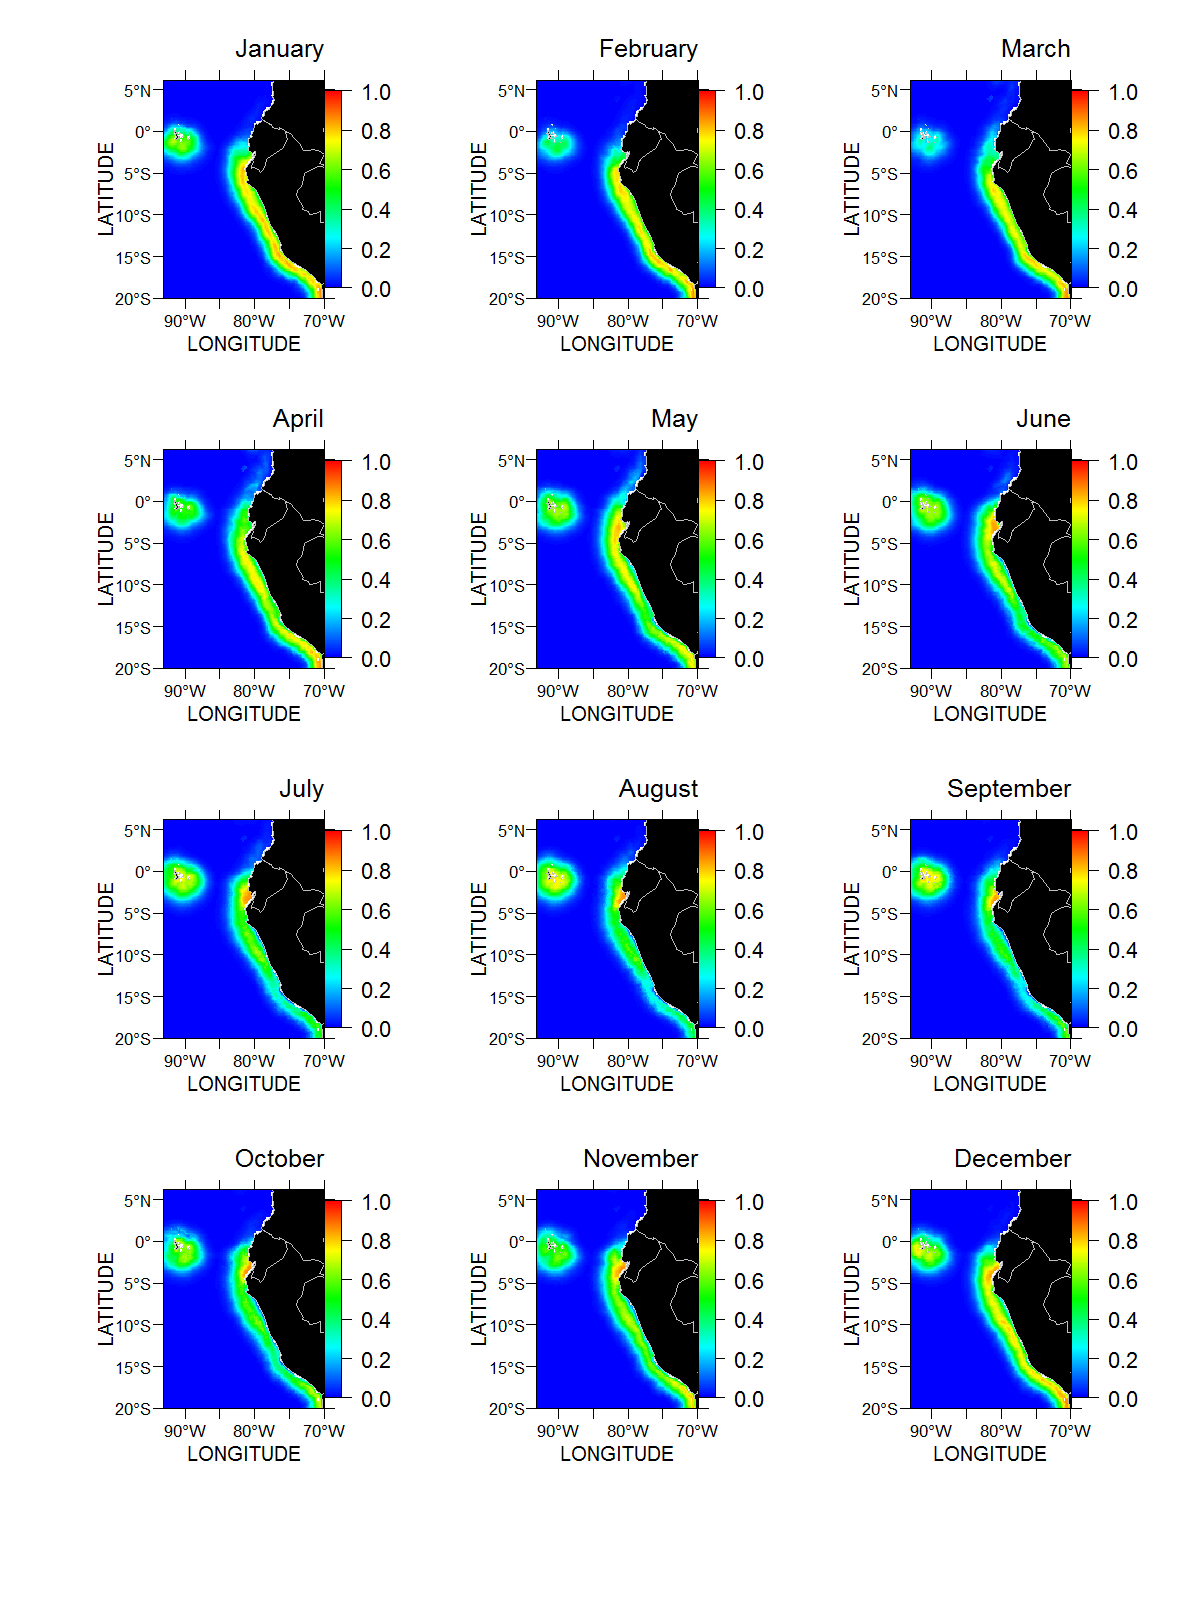
\includegraphics[height=0.8\textheight]{figures/caballa-climatology}
\caption[Seasonal patterns of the distribution of mackerel]{Seasonal patterns of the distribution of mackerel as predicted by the species distribution models used to build the interannual maps for the NHCE OSMOSE model.}
\label{fig:caballa-climatology}
\end{figure}

\begin{figure}
\centering
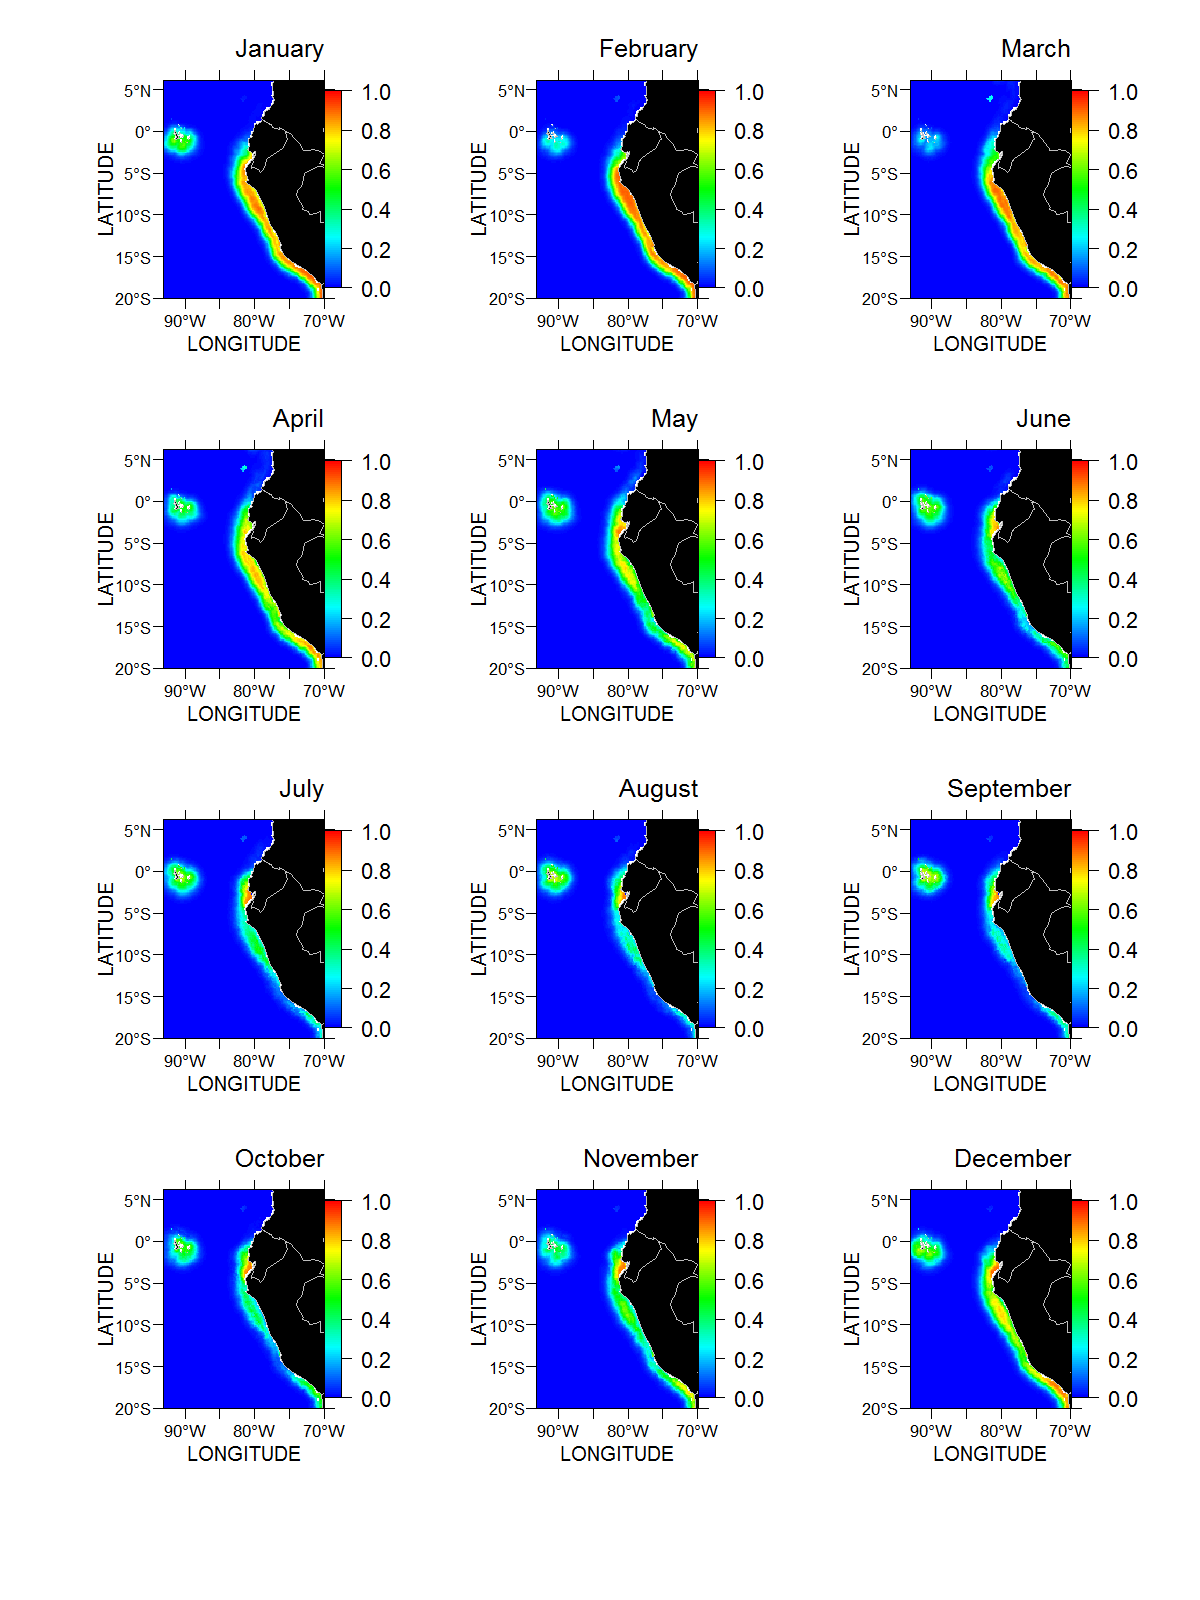
\includegraphics[height=0.8\textheight]{figures/sardine-climatology}
\caption[Seasonal patterns of the distribution of Peruvian anchovy]{Seasonal patterns of the distribution of sardine as predicted by the species distribution models used to build the interannual maps for the NHCE OSMOSE model.}
\label{fig:sardine-climatology}
\end{figure}


\section*{References}

Aumont O. and Bopp L. 2006. Globalizing results from ocean in situ iron fertilization studies. Gl.Biogeochem.Cyc. 20:GB2017.

Budgell, W.P., 2005: Numerical simulation of ice-ocean variability in the Barents Sea region, Ocean Dynamics, DOI 10.1007/s10236-005-0008-3.

Cambon G.,Goubanova K., Marchesiello P., et al. 2013. Assessing the impact of downscaled atmospheric winds on a regional ocean model simulation of the Humboldt system. Ocean Modelling 65:11-24.

Colas, F., X. Capet, J. C. McWilliams, et al. 2008. 1997–1998 El Nino off Peru: A numerical study. Prog. Oceanogr.79:138–155.

Da Silva A.M., Young C.C. Levitus S. 1994. Atlas of surface marina data 1994. Technical report, Natl. Oceanogr. And Atmos. Admin. Silver Spring Md.

Di Lorenzo, E., 2003: Seasonal dynamics of the surface circulation in the southern California Current System, Deep-Sea Res., Part II, 50, 2371-2388.

Dinniman, M. S., J. M. Klinck, and W. O. Smith Jr. (2003), Cross shelf exchange in a model of the Ross Sea circulation and biogeochemistry, Deep-Sea Res., Part II, 50, 3103-3120.

Echevin V., Goubanova K., Dewitte B., A., et al. 2012. Sensitivity of the Humboldt Current system to global warming: a downscaling experiment of the IPSL-CM4 model. Clim. Dyn. 38(3-4):761-774.

Espinoza-Morriberón D. 2012. Impacto de la circulaciónecuatorialen la zonamínima de oxígenopresenteen el nortedelEcosistema de la Corriente de Humboldt.Thesis to obtain the degree of Master in Marine Sciences. Unidad de PostgradoVíctorAlzamora. Facultad de Ciencia y Filosofía. Universidad PeruanaCayetano Heredia, Lima. 115 pp.

Espinoza-Morriberón D., Echevin V., Romero Y.,  Ledesma J., Oliveros-Ramos R., Tam J., (submitted) Validation of ROMS-PISCES Coupled Model in the Southeast Pacific. Part II: Biogeochemical conditions.

Gruber N., Frenzel H., Doney S.C., et al. 2006. Eddy-resolving simulation of plankton ecosystem dynamics in the California Current System. Deep Sea Res. 1(53): 1483-516.

Haidvogel, D. B., H. G. Arango, K. Hedstrom, A. Beckmann, P. Malanotte-Rizzoli, and A. F. Shchepetkin (2000), Model evaluation experiments in the North Atlantic Basin: Simulations in nonlinear terrain-following coordinates, Dyn. Atmos. Oceans, 32, 239-281.

Montes I., Colas F., Capet X., et al. 2010. On the pathways of the equatorial subsurface currents in the eastern equatorial Pacific and their contributions to the Peru Chile Undercurrent. J. Geophys. Res. 115: C09003.

Penven P., Echevin V, Pasapera J, et al. 2005. Average circulation, seasonal cycle, and mesoscale dynamics of the Peru Current System: A modeling approach. J. Geophys. Res. 110: C10021. DOI:10.1029/2005JC002945.

Redfield A.C., Ketchum B.H. and Richards F.A. 1963. The influence of organisms on the composition of the sea-water. En: Hill M.N. (Eds.). Interscience 2: 26-77.

Risien C.M. and Chelton D.B. 2008. A Global Climatology of Surface Wind and Wind Stress Fields from Eight Years of QuikScatscatterometer Data. J. Phys. Oceanogr. 38: 2379-2413.

Romero Y., Espinoza-Morriberón D., Oliveros-Ramos R., Tam J., Echevin V. (submitted) Validation of ROMS-PISCES Coupled Model in the Southeast Pacific. Part I: Physical conditions.

Peliz, A., J. Dubert, D. B. Haidvogel, and B. Le Cann (2003), Generation and unstable evolution of a density-driven Eastern Poleward Current: The Iberian Poleward Current, J. Geophys. Res., 108(C8), 3268, doi:10.1029/2002JC001443.

Shchepetkin, A.F., McWilliams, J.C., 2005. Regional Ocean Model System: a split-explicit ocean model with a free-surface and topography-following vertical coordinate. Ocean Modelling 9, 347-404.

Warner, J.C, C.R. Sherwood, H.G. Arango, and R.P. Signell (2005) Performance of four Turbulence Closure Methods Implemented using a Generic Length Scale Method. Ocean Modelling, 8, 81-113.

Wilkin, J.L., H.G. Arango, D.B. Haidvogel, C.S. Lichtenwalner, S.M. Durski, and K.S. Hedstrom, 2005: A regional Ocean Modeling System for the Long-term Ecosystem Observatory. J. Geophys. Res., 110, C06S91, doi:10.1029/2003JC002218.


\cleardoublepage

\chapter{On the calibration of ecosystem models using time series data} 
\label{EA}
\thispagestyle{empty}%
% how to calibrate an ecosystem model
An original Evolutionary Algorithm has been developed during the thesis for the purpose of calibrating complex stochastic models. The concepts and details are provided in section \ref{AHR-ES}.

This optimization algorithm and the tools related to the calibration of ecological models have been implemented in an R package, \texttt{calibrar}, which is also described in this chapter (manuscript 2).


\section[An evolutionary algorithm for the calibration of ecological models]{An evolutionary algorithm for the calibration of ecological models using maximum likelihood estimation}
\label{AHR-ES}

Evolutionary algorithms (EA) are computer programs designed for the automatic solving of complex problems such as minimization of functions, and are inspired by the process of Darwinian evolution (Jones 1998). The three main types of EA are Genetic Algorithms (GA), Evolutionary Programming (EP) and Evolutionary Strategies (ES). Historically, Evolutionary Programming and especially Genetic Algorithms were designed with a broader range of applications (B\"ack and Schewefel, 1993) while Evolutionary Strategies (ESs) were specifically designed for parameter optimization problems (Jones, 1998). 
For optimization problems, EAs work over a population of ``individuals'' searching over the space of solutions. Each individual encodes a solution (e.g. a vector of parameter values for a model) to the problem which performance can be assessed. 
EAs rely on three main processes: selection, recombination and mutation. The selection process is intended to select the individuals which will produce offspring (i.e the population for the next generation). The recombination process allows inbreeding the selected individuals (parents) in an attempt to enhance their performance. Finally, the mutation process produces random variability in the population, normally by modifying the solution encoded by the parents. 

The next sections describe the material presented in the Supplementary material 1 of the manuscript presented in section \ref{paper2}

\subsection{Evolutionary strategies}

In ESs, selection and recombination are deterministic parametric processes. Additionally, EAs include some ?meta-parameters? controlling the behavior of the algorithm itself (e.g. the mutation rates). ESs also include ``self-adaptation'' procedures allowing to make the meta-parameters of the algorithm vary to improve their performance over the evolutionary process. ESs focus on mutation as the main search operator, and it has been pointed out that it is necessary to use recombination in connection to self-adaptation to improve the performance of the algorithm (Thomas and Schewefel, 1993). A comprehensive synthesis of Evolutionary Strategies can be found in Beyer and Schwefel (2002). 

We consider a population $\{x_i\}$, with $x_i \in \RR^n$, for $i=1, \dots,  \lambda$ and $n$ the dimension of the problem (i.e the number of parameters to estimate). We also need to define an objective function $f$ (so called fitness function) to be minimized. So, for each $x_i$ we can calculate $f(x_i)$ and we can sort the individuals of the population by their fitness values:
\begin{equation}
f(x_{1:\lambda}) \leq f(x_{2:\lambda}) \leq \dots \leq f(x_{\lambda:\lambda})
\label{eq-sort}
\end{equation}
Where $x_{i:\lambda}$ encodes the $i$-th lower value for the function $f$ among the population. This allows us to carry on the selection of the best $\mu < \lambda$ individuals of the population, which will constitute the parents for the next generation. 

The recombination of the parents can follow different rules. It can be as simple as taking the mean (or weighted mean) of the $\mu$ selected parents. Finally, the mutation process is used to produce a new generation, for example by sampling the new $x_i$ from a multivariate normal distribution:

$$x_i \sim N(m, C)$$

\noindent where $m$ is an $n$-dimensional vector resulting from the recombination of the parents and $C$ is a covariance matrix. During the course of the evolutionary process, $m$ will converge to an optimal solution. 

In the algorithm developed in this work, we introduce a new method for an adaptative hierarchical recombination (AHR), optimized for parameter estimation of models using several sources of information (i.e calibration using several sources of data). 
% define self adaptation
Additionally, in order to improve the convergence and search capabilities, we implement self-adaptation procedures  to improve the adaptation of the covariance matrix $C$ during the optimization. 

In order to introduce a self-adaptation process in our algorithm, we assume $C$ is a diagonal matrix, while extending the results to a generic covariance matrix is a work under progress. In the next section, the algorithm developed is described in detail.

\subsection{The AHR-ES Algorithm}

\subsubsection{Objective function}

We are considering a general class of objective functions $f$:

\begin{equation}
f(x) = f_0(x) + \sum_{k=1}^K f_k(x),
\end{equation}

\noindent where $x \in \RR^n$ is a parameter vector and $f_k$, $k=0,\ldots, K$ are the \emph{partial fitnesses}. The objective of the calibration is to optimize $f(x)$, the search being directed by the recombination between individuals with ``local'' success (optimizing $f_k$, $k=1,\ldots, K$). 

It is important to notice that we are not sorting the parents according to the partial fitness for the $f_0$ component, but this component contributes to the total fitness and the initial selection.
In particular, $f_k$ could be the likelihood function associated to each calibration variable. By using likelihood functions, it is straightforward to build fitness functions to calibrate variables with data time series. Also, this choice makes a handful of statistical procedures available to test the goodness of fit, to estimate confidence intervals, etc. On the other hand, likelihood fitness functions could be very complex and highly multimodal, especially when handling a model with non-linear relationships and stochasticity. Optimizing likelihood functions for complex models could be prone to premature stagnation and requires more generations to find optimal solutions, reason why it is important to reduce population sizes (to reduce computing time) and to use properly defined self-adapted mutation rates (to increase rate of convergence).

\subsection{Selection}

We select the $\mu<\lambda$ parents $\xpar_i$ ($i=1, \dots, \mu$) which have the lowest value of the objective function $f$.
 Then, for each partial fitness $f_i$ ($i=1, \dots, K$) we will sort the parents as in Equation~\eqref{eq-sort}:
 
\begin{equation}
f_k(\xpar_{1:\mu,k}) \leq f_k(\xpar_{2:\mu,k}) \leq \dots \leq f_k(\xpar_{\mu:\mu,k})
\label{eq-sort2}
\end{equation}

\noindent for each $m=1, \dots, K$ partial fitness.

\subsection{Recombination}

As a first step, we will recombine the parents according to their success at optimizing each partial fitness $f_k$, given a set of weights $w_i$ ($i=1, \dots, \mu$):

\begin{eqnarray}
\xmean& = & \textstyle \sum_iw_i \xpar_{i:\mu, m}\\ 
\smean^2 & = & \textstyle \sum_iw_i\xpar_{i:\mu, m}^2 - \xmean^2
\end{eqnarray}

\noindent such that $w_i \geq w_j$ for $i<j$ and $\sum_iw_i =1$. Note that $\xmean^2$ is taken entry--wise, i.e. squaring each component of $\xmean$ independently (Hadamard product). This initial recombination allows to better use the information in all selected individuals, and particulary to reduce the impact of selecting an individual with a good fitness value just by chance, especially when dealing with stochastic models. As part of the recombination we also calculate $\smean$ which provides information about the variability of each parameter value among the parents.

Then, we exploit all the historical information on $\xmean$ and $\smean$ by exponentially weighting the past of the recombined parents:
\begin{eqnarray}
\xdyn(g) & = & \left(1-\alpha\right)\xdyn(g-1) + \alpha\xmean\\
\sdyn^2 (g) & = & \left(1-\alpha\right)\left(\xdyn^2(g-1) + \sdyn^2(g-1)\right) + \alpha\left(\smean^2 + \xmean^2\right) - \xdyn^2(g) 
\end{eqnarray}
\noindent for each $m=1, \dots, K$ partial fitness, and generation $g$. Here, $\xdyn(g)$ and $\sdyn(g)$ are calculated as moving average and variance for generation $g$, to take into account past information with exponentially decreasing weights given by $\alpha \in [0,1]$, a meta-parameter of the algorithm, which controls the rate at which the algorithm learns from the current parents. Particularly, $\sdyn$ provides information on how important a particular parameter is for the minimization of the objective function, since the more important the parameter the smaller the variability that we would expect across the generations.
Now, let's define $\smin=\min_n\sdyn$ and $\smax=\max_n\sdyn$, the minimum and maximum over the $n$ entries of $\sdyn$, respectively to calculate:

\begin{equation}
\hat{w}_k = \left[\frac{\smax-\sdyn}{\smax-\smin}\right]^\beta
\end{equation} 

\begin{equation}
w_k =\frac{\hat{w}_k}{\|\hat{w}_k\|_1} 
\end{equation} 


\noindent for $\beta \geq 1 $, and $\|\hat{w}_k\|_1$ is the $L_1$ norm of $\hat{w}_k$, taken to make the sum of $w_k$ equal to 1. Again, the quotient and the power are taken entry--wise . $w_k$ ponderates the relative importance of each parameter to the partial fitness $m$. When parameters are bounded, the vector $\sdyn$ can be divided by the ranges of each parameter before the recombination stage for rescaling purposes.

Finally, we recombine all parents to produce the \emph{parental genotype} $\xfinal$ by using the weights given by $w_k$ and the first recombined parents given by $\xdyn$:

\begin{equation}
\xfinal[i] = \frac{\sum_{m=1}^M w_k[i]\xdyn[i]}{\sum_{m=1}^M w_k[i]},
\label{eq-final_recombination}
\end{equation}

\noindent where $i=1, \dots, n$ represents the position of a particular parameter in the vectors.

This final recombination uses dynamically changing weights which take into account the variability of each parameter independently and its importance to minimize every partial component of the objective function.  

\subsection{Mutation}

The new individuals of the population in generation $g+1$ will be produced by mutating the parental genotype $\xfinal$ using a multivariate normal distribution:

\begin{equation}
x_i^{(g+1)} \sim N(\xfinal^{(g)}, \step^{(g)}C^{(g)})
\end{equation}

\noindent for $i=1, \dots, \lambda$. The matrix $C^{(g)}$ is constructed following the self-adaptation algorithm techniques (Covariance Matrix Adaptation CMA-ES; Hansen and Ostermeier 2001) and $\step$ is the step size control calculated as in  
Hansen and Ostermeier (2001). The reader can read the source code for details on this particular implementation.

Additionally, when the parameters are bounded, a truncated multivariate normal distribution is used for the mutation process instead of a multivariate normal distribution. 



\section{calibrar: an R package for the calibration of ecological models}
\label{calibrar}

In this section we include a manuscript submitted to the journal ``Methods in Ecology an Evolution'' (manuscript MEE-14-10-625).

\includepaper{papers/oliveros_shin-mee-calibrar_for_thesis.pdf}
\includeappendix{papers/oliveros_shin-mee-calibrar_S2.pdf}

\cleardoublepage

\chapter{Parameterization and calibration of the end-to-end ROMS-PISCES-OSMOSE model of the Northern Humboldt Current Ecosystem} 
\label{calibration}
\chaptermark{Calibration of the E2E model ROMS-PISCES-OSMOSE of the NHCE}
\thispagestyle{empty}%


In this chapter we address the key calibration phase of the end-to-end (E2E) ecosystem model ROMS-PISCES-OSMOSE for the Northern Humboldt Current Ecosystem. For this purpose, we highlight some issues related to the confrontation of complex ecosystem models to data and propose a methodology for a sequential multi-phases calibration of ecosystem models (section \ref{paper1}). We first propose two criteria to classify the parameters of a model: the model dependency and the time variability of the parameters. Then, these criteria and the availability of approximate initial estimates are used as decision rules to determine which parameters need to be estimated, and their precedence order in the sequential calibration process. 

The E2E model is calibrated using an the evolutionary algorithm described in chapter \ref{EA} and a likelihood approach to fit monthly time series data of landings, abundance indices and catch at length distributions from 1992 to 2008.  

\section{A sequential approach for the calibration of ecosystem models}
\label{paper1}

In this section we include a manuscript submitted to the journal ``Progress in Oceanography'' (manuscript PROOCE-S-14-00115).


\includepaper{papers/oliveros_etal-PiO-sequential_calibration_for_thesis.pdf}



\cleardoublepage

%\chapter{Applications of ROMS-PISCES-OSMOSE model to fishery management in the Humboldt Current Ecosystem}
%\chaptermark{Applications of the ROMS-PISCES-OSMOSE to fishery management} 
%\thispagestyle{empty}%
%\lipsum[1-2]

\section{Maximum sustainable yields in an ecosystem context}
\lipsum[1-5]

\section{Assessing the impact of fishing in the ecosystem}
\lipsum[6-10]

\section{Comparison with single stock assessment models}
\lipsum[11-15]
%\cleardoublepage

\chapter*{Concluding remarks and perspectives} 
\thispagestyle{empty}%
\addcontentsline{toc}{chapter}{Concluding remarks and perspectives}
\markboth{General conclusions and perspectives}{} 

\section*{Confronting ecosystem models to data}

Confronting ecosystem models to data is essential to increase their credibility and to start using them in support to management decision. A successful model calibration implies several computational, theoretical and practical challenges. The \texttt{calibrar} R package intends to provide a framework to simplify the calibration of complex models, in particular stochastic ones, for which fewer developments have been done compared to those for deterministic and differentiable models. There is “no free lunch” in optimization, and no optimization algorithm will perform bestfor every type of optimization problems (Wolpert and Macready 1997). In this direction, the next step we envisage is the inclusion of other optimization algorithms in our \texttt{calibrar} package so the users are provided with a suite of tools to solve a variety of calibration problems in a transparent way without additional technical complications. In parallel, more tests with other models and real-world calibration problems are required to improve the generality of the package, its flexibility and the robustness of the optimization algorithm. 


However, calibration is only one step in the process of rigorous model development and application. One important step we did not prioritize here due to time constraints, is a full sensitivity analysis for the OSMOSE model, which could have greatly helped in the calibration process by providing a rationale to reduce the number of parameters to estimate (Megrey et al. 2007, Dueri et al. 2012, Lehuta et al 2013). Complementary to this first approach and expected to be developed in close future is an uncertainty analysis on the parameters of the E2E model, relying on the calibration phase but also on the analysis of the uncertainties due to the different component models (ROMS-NPZD, OSMOSE, climate niches) and how they can combine together into an assessment of different management scenarios in the HCE. Additionally, a successful calibration does not mean that a model is reliable (Gaume et al. 1998), and a proper validation is always required, eventually providing information to improve the model and to revise the calibration (Walter and Pronzato 1997, Jorgensen and Bendoricchio 2001). In particular, a more detailed validation of our model results including alternative sources of information (e.g. trophic ecology) could help to increase the credibility of the model. 

\section*{Bridging ecosystem models with single species models}

Management strategy evaluation (MSE) is a set of simulation-based procedures to compare alternative management procedures (Butterworth 2007, De Lara and Martinet, 2008). More precisely, MSE consists in defining a set of operational objectives and to evaluate, by means of simulations, the performance of alternative management procedures in relation to the set of objectives defined, and taking into account the uncertainties related to the modeling process (Sainsbury et al. 2000, Butterworth 2007). One of the weakest points in some MSE applications is the use of the same model as the operative model (used to generate artificial data) and the assessment model (used to evaluate the status of the population given the artificial data generated by the assessment model). Even if the operative model is a more complex version of the assessment model, it is likely that the results would be artificially better than if an independent model with a different structure was used to generate the data. Additionally, by doing so, it is implicit that the assumptions of the model are correct, i.e. the reality is driven by the processes included in the operative model, which can lead to important model misspecifications and bias in the MSE because model uncertainty would not have been taken into account. In particular, when using single-species models as operative models, the impact of species interactions and their variability is not taken into account (or at least not directly) which could bias long term projections. In this respect, future MSE in the HCE could rely on a fully calibrated ecosystem model as the operative model while still using the current single-species assessment models for management purposes.  


A weakness of some single-species models is to take as constants some parameters which are expected to have a strong variability, like natural mortality, which greatly depends on the changes in the environmental conditions and trophic structure of the ecosystem, as well as the life stage of the individuals. Ecosystem models can provide information about such variability, which can be incorporated as a forcing or additional source of uncertainty in single-species models. By doing so, it would be possible to understand the impact of other sources of variability (e.g. the environment) in single-species models, which normally rely on the (phenomenological) estimation of time series of deviates to incorporate the impact of such sources of variability. On the other hand, keeping multi- and single-species models independent (not using outputs from one as input to the other) allows us to provide insights into the impact of different assumptions and resolution of the model processes and structure, e.g. single-species models being more fishery oriented (e.g selectivity modeling) and ecosystem models being more trophic oriented (e.g. predation modeling). 


\section*{Applications to EBFM}


Despite some attempts to move towards EBFM around the world, most commercial species remain managed using single-species management procedures (MP). Therefore, one interesting application would be to evaluate the impact of neglecting the interspecific interactions in the ecosystem as well as the interactions between single species MPs leading to concrete multispecies management strategies. This can be done by replicating the single-species management procedures using ecosystem models to eventually help to develop more robust MPs in an ecosystem context. Additionally, current single-species reference points (RP) cannot take into account important ecosystem processes, particularly here in the HCE the environmentally-induced changes in the ecosystem structure. Ecosystem models will allow to estimate ecosystem RPs taking into account the complex dynamics of the ecosystems while simultaneously allowing to work in a single-species context. However, by counting with ecosystem-based RPs (like multi-species MSY) and operational ecosystem models, a further step would be to carry out an integrated ecosystem MSE. Since several criteria are used to estimate "optimal" strategies for fisheries management, but most of them rely on single-species models, the solutions under the same criteria can be totally different by considering an ecosystem approach. Furthermore, ecosystem models can be better at forecasting the impacts of the environmental variability in the dynamics of exploited populations. Currently, physical models can provide synthetic scenarios of natural and human-induced environmental variability which can be used for MSE purposes. On the other hand, single-species models normally need to rely on simpler time-series of environmental variability to force the models, while spatial ecosystem models, like OSMOSE, can better exploit the variability given by ocean and biogeochemical models.


\section*{OSMOSE modelling platform}


The version of OSMOSE implemented in this thesis (OSMOSE 3 release 1, \url{www.osmose-model.org}) includes several improvements with respect to the versions used in previous published applications (OSMOSE 2), particularly related to the incorporation of interannual variability in the model. The OSMOSE model for the NHCE is also the first interannual application using OSMOSE. However, in all OSMOSE versions, the impact of fishing is simplified as it does not explicitly handle multiple fisheries but just species catches or fishing mortalities. OSMOSE 3 includes more flexible selectivity specifications (in addition to the original knife-edge selectivity), but a more general approach is needed to explore options for real management applications in a multiple fisheries context, e.g. one species being targeted by more than one fisheries (possibly in different areas) and one fishery targeting more than one species (possibly, with different selectivities and catchabilities). This approach will lead fisheries to be modeled similarly to other predator species which can have access to all the other species inside the limits specified by the size-specific predation hypothesis of OSMOSE.


Another improvement to bringing OSMOSE to better represent the NHCE ecosystem dynamics is a finer specification of land-based predators, like mammals and birds. This can be handled in OSMOSE 3 by using a time-varying size-specific natural mortality instead of a constant one as is the case in the current implementation. This approach will need to specify i) a proxy of the natural mortality induced by the land-based predators (e.g. time series of abundance or consumption), ii) the shape of the selectivity of the predator (equivalent to the ratios for the size-dependent predation for other predators), iii) the target preys (equivalent to the accessibility matrix for other predators) and iv) the estimation of the average natural mortality induced by the land-based predators during the calibration process. For example, data is available in the NHCE to apply such approach for seabirds preying upon anchovy. Other possibility for the inclusion of land-based predators is to assimilate their parameterization to that of a "fishery" in a multi-fisheries implementation as discussed before.


Finally, the interannual implementation of OSMOSE required to model the spatial distribution of fish, which is one of the current forcings in OSMOSE, and to construct interannual maps of fish distributions. However, fish spatial distribution is currently disrupted as discrete maps drive fish spatial dynamics. To reduce the potential disruptive effect, we refined the forcing by using seasonal maps for most of the species (four maps per year), but further details and mechanisms should be included in the movement sub-model in OSMOSE, particularly to smooth the transitions between maps and to not lose the spatial structure created in the model.


\section*{HCE modelling} 


A model cannot be better than the information used to build it. Ecosystem models in particular rely on a great quantity and quality of information in order to be able to properly reproduce the observed dynamics of the ecosystem and identify the parameters of the model. In this sense, gathering the information needed to build an interannual OSMOSE model for the Northern Humboldt Current Ecosystem was by itself a complex task, requiring a lot of pre-processing work in terms of data standardization. To review and standardize the information needed for this application has motivated the launch of an on-going IMARPE project ("Estimation of fishery-biological parameters for the sustainable management of marine resources", funded by RM-350-2013-PRODUCE) that has the objective to improve the IMARPE's database (IMARSIS) and to digitalize and concentrate all the sources of information pertinent for modeling purposes. Also, improvements in the standardization of abundance indices are needed, as the main source of information on the variability of the exploited populations. Currently, two master theses are under way at IMARPE to address i) a review of the fishery-independent abundance indices for Jack mackerel and ii) the development of empirical echo-abundance indices when length data from surveys is not appropriate to estimate biomass from acoustic data, mainly for less common non-commercial species.


In terms of the spatial distribution modelling, the current implementation of OSMOSE-NHCE uses the same distribution for all the schools of the same species, independently of the age or size. As data exist for different stages of anchovy (larvae, juveniles, recruits and adults), another master thesis is in progress to refine the spatial distribution models. Also, munida (squad lobster) requires more detailed modeling of its spatial distribution since the larger individuals start to develop demersal habits in comparison to the smaller ones which are pelagics off Peru. Finally, a more detailed pattern oriented validation is needed for all modelled species to ensure that the maps produced fulfill the requirements for our modeling objectives.


\section*{References}

De Lara M. and Doyen L. 2008. Sustainable Management of Natural Resources. Mathematical Models and Methods. Springer-Verlag, Berlin, 2008.

Dueri S., Faugeras  B., Maury O.,2012. Modelling the skipjack tuna dynamics in the Indian Ocean with APECOSM-E – Part 2: Parameter estimation and sensitivity analysis. Ecological Modelling 245:55-64.

Gaume E., Villeneuve J.-P., Desbordes M., 1998. Uncertainty assessment and analysis of the calibrated parameter values of an urban storm water quality model. Journal of Hydrology 210: 38–50.

Lehuta S., Petitgas P., Mahévas S., Huret M., Vermard Y., Uriarte A.,  Record N.R.,2013. Selection  and  validation  of  a  complex  fishery  model  using  an  uncertainty hierarchy. Fisheries Research  143:57–  66.

Jorgensen S.E. and Bendoricchio G., 2001. Fundamentals of Ecological Modelling. Third Edition. Elsevier. 530pp.

Megrey B.A., Rose K.A, Klumb R.A, Hay D.E, Werner F.E, Eslinger D.L, Smith S.L., 2007. A bioenergetics-based population dynamics model of Pacific herring (Clupeaharenguspallasi) coupled to a lower trophic level nutrient-–phyto\-plankton–-zoo\-plankton model: Description, calibration, and sensitivity analysis. Ecological Modelling 202:144–164.

Sainsbury K. J., Punt A. E. and Smith A. D. M. 2000. Design of operational management strategies for achieving fishery ecosystem ob¬jectives. ICES Journal of Marine Science, 57: 731-741.

Walter E. and Pronzato L., 1997. Identification of parametric models from Experimental data. Springer Masson. 413pp.

Wolpert, D.H. and Macready, W.G. (1997) No Free Lunch Theorems for Optimization. IEEE Transactions on Evolutionary Computation, 1(1):67-82.


 
\cleardoublepage

\cleardoublepage        % asegura que el nro de página sea correcto en la ToC.
%\phantomsection  % Para que hyperref apunte a la página correcta

%\addcontentsline{toc}{chapter}{Bibliography}
% \bibliography{references.bib} \thispagestyle{empty}%
%  \printbibliography

%      \let\normalsize\small
%     \appendix
%     \small
%     
% \appendix
%\cleardoublepage
%\appendix
%\appendixpage \thispagestyle{empty}%
%\noappendicestocpagenum
%\addappheadtotoc

%\begin{appendices}
%
%\chapter{Publications, manuscripts and presentations}
%\thispagestyle{empty}%
%\section{Publications}
\lipsum[1]

\section{Manuscripts}
\lipsum[1]

\section{Presentations at International Conferences}
\lipsum[1]


%\cleardoublepage
%
%\chapter{Scientific Software}
%\thispagestyle{empty}%
%\lipsum[1-2]

\section{calibrar}
\lipsum[3]

\section{osmose2R}
\lipsum[4]

\section{kali}
\lipsum[5]


%\cleardoublepage
%
%
%\end{appendices}

\backmatter


\end{document}
